%% Copernicus Publications Manuscript Preparation Template for LaTeX Submissions
%DIF LATEXDIFF DIFFERENCE FILE
%DIF DEL version_2402/viirs_article_tc_new/main.tex   Thu Mar 12 20:06:43 2026
%DIF ADD viirs_paper/main.tex                         Thu Jul 23 10:44:05 2026
%% ---------------------------------
%% This template should be used for copernicus.cls
%% The class file and some style files are bundled in the Copernicus Latex Package, which can be downloaded from the different journal webpages.
%% For further assistance please contact Copernicus Publications at: production@copernicus.org
%% https://publications.copernicus.org/for_authors/manuscript_preparation.html


%% Please use the following documentclass and journal abbreviations for preprints and final revised papers.

%% 2-column papers and preprints
\documentclass[tc, manuscript]{copernicus}



%% Journal abbreviations (please use the same for preprints and final revised papers)


% Advances in Geosciences (adgeo)
% Advances in Radio Science (ars)
% Advances in Science and Research (asr)
% Advances in Statistical Climatology, Meteorology and Oceanography (ascmo)
% Aerosol Research (ar)
% Annales Geophysicae (angeo)
% Archives Animal Breeding (aab)
% Atmospheric Chemistry and Physics (acp)
% Atmospheric Measurement Techniques (amt)
% Biogeosciences (bg)
% Climate of the Past (cp)
% DEUQUA Special Publications (deuquasp)
% Earth Surface Dynamics (esurf)
% Earth System Dynamics (esd)
% Earth System Science Data (essd)
% E&G Quaternary Science Journal (egqsj)
% EGUsphere (egusphere) | This is only for EGUsphere preprints submitted without relation to an EGU journal.
% European Journal of Mineralogy (ejm)
% Fossil Record (fr)
% Geochronology (gchron)
% Geographica Helvetica (gh)
% Geoscience Communication (gc)
% Geoscientific Instrumentation, Methods and Data Systems (gi)
% Geoscientific Model Development (gmd)
% History of Geo- and Space Sciences (hgss)
% Hydrology and Earth System Sciences (hess)
% Journal of Bone and Joint Infection (jbji)
% Journal of Micropalaeontology (jm)
% Journal of Sensors and Sensor Systems (jsss)
% Magnetic Resonance (mr)
% Mechanical Sciences (ms)
% Natural Hazards and Earth System Sciences (nhess)
% Nonlinear Processes in Geophysics (npg)
% Ocean Science (os)
% Polarforschung - Journal of the German Society for Polar Research (polf)
% Primate Biology (pb)
% Proceedings of the International Association of Hydrological Sciences (piahs)
% Safety of Nuclear Waste Disposal (sand)
% Scientific Drilling (sd)
% SOIL (soil)
% Solid Earth (se)
% State of the Planet (sp)
% The Cryosphere (tc)
% Weather and Climate Dynamics (wcd)
% Web Ecology (we)
% Wind Energy Science (wes)


% \usepackage commands included in the copernicus.cls:
%\usepackage[german, english]{babel}
\usepackage{tabularx}
\usepackage{cancel}
\usepackage{multirow}
\usepackage{supertabular}
\usepackage{algorithmic}
\usepackage{algorithm}
\usepackage{amsthm}
\usepackage{float}
\usepackage{subfig}
\usepackage{rotating}
\usepackage{array}
\usepackage{hyperref}


\newcolumntype{R}[1]{>{\raggedleft\let\newline\\\arraybackslash\hspace{0pt}}m{#1}}
%DIF PREAMBLE EXTENSION ADDED BY LATEXDIFF
%DIF UNDERLINE PREAMBLE %DIF PREAMBLE
\RequirePackage[normalem]{ulem} %DIF PREAMBLE
\RequirePackage{color}\definecolor{RED}{rgb}{1,0,0}\definecolor{BLUE}{rgb}{0,0,1} %DIF PREAMBLE
\providecommand{\DIFaddtex}[1]{{\protect\color{blue}\uwave{#1}}} %DIF PREAMBLE
\providecommand{\DIFdeltex}[1]{{\protect\color{red}\sout{#1}}}                      %DIF PREAMBLE
%DIF SAFE PREAMBLE %DIF PREAMBLE
\providecommand{\DIFaddbegin}{} %DIF PREAMBLE
\providecommand{\DIFaddend}{} %DIF PREAMBLE
\providecommand{\DIFdelbegin}{} %DIF PREAMBLE
\providecommand{\DIFdelend}{} %DIF PREAMBLE
\providecommand{\DIFmodbegin}{} %DIF PREAMBLE
\providecommand{\DIFmodend}{} %DIF PREAMBLE
%DIF FLOATSAFE PREAMBLE %DIF PREAMBLE
\providecommand{\DIFaddFL}[1]{\DIFadd{#1}} %DIF PREAMBLE
\providecommand{\DIFdelFL}[1]{\DIFdel{#1}} %DIF PREAMBLE
\providecommand{\DIFaddbeginFL}{} %DIF PREAMBLE
\providecommand{\DIFaddendFL}{} %DIF PREAMBLE
\providecommand{\DIFdelbeginFL}{} %DIF PREAMBLE
\providecommand{\DIFdelendFL}{} %DIF PREAMBLE
%DIF HYPERREF PREAMBLE %DIF PREAMBLE
\providecommand{\DIFadd}[1]{\texorpdfstring{\DIFaddtex{#1}}{#1}} %DIF PREAMBLE
\providecommand{\DIFdel}[1]{\texorpdfstring{\DIFdeltex{#1}}{}} %DIF PREAMBLE
%DIF LISTINGS PREAMBLE %DIF PREAMBLE
\RequirePackage{listings} %DIF PREAMBLE
\RequirePackage{color} %DIF PREAMBLE
\lstdefinelanguage{DIFcode}{ %DIF PREAMBLE
%DIF DIFCODE_UNDERLINE %DIF PREAMBLE
  moredelim=[il][\color{red}\sout]{\%DIF\ <\ }, %DIF PREAMBLE
  moredelim=[il][\color{blue}\uwave]{\%DIF\ >\ } %DIF PREAMBLE
} %DIF PREAMBLE
\lstdefinestyle{DIFverbatimstyle}{ %DIF PREAMBLE
	language=DIFcode, %DIF PREAMBLE
	basicstyle=\ttfamily, %DIF PREAMBLE
	columns=fullflexible, %DIF PREAMBLE
	keepspaces=true %DIF PREAMBLE
} %DIF PREAMBLE
\lstnewenvironment{DIFverbatim}{\lstset{style=DIFverbatimstyle}}{} %DIF PREAMBLE
\lstnewenvironment{DIFverbatim*}{\lstset{style=DIFverbatimstyle,showspaces=true}}{} %DIF PREAMBLE
%DIF END PREAMBLE EXTENSION ADDED BY LATEXDIFF

\begin{document}

\title{Assessing \DIFdelbegin \DIFdel{VIIRS constellation seasonal }\DIFdelend snow cover \DIFdelbegin \DIFdel{over }\DIFdelend \DIFaddbegin \DIFadd{products from }\DIFaddend the \DIFdelbegin \DIFdel{French mountains }\DIFdelend \DIFaddbegin \DIFadd{VIIRS constellation under varying topographic and seasonal conditions }\DIFaddend with Sentinel-2}



% \Author[affil]{given_name}{surname}

\Author[1][nicola.imperatore@meteo.fr]{Nicola}{Imperatore} %% correspondence author
\Author[2]{Simon}{Gascoin}
\Author[1]{Matthieu}{Lafaysse}
\Author[1]{Marie}{Dumont}
\Author[3]{Adrien}{Mauss}
\Author[3]{Stéphane}{Guével}
\Author[3]{Jean-Baptiste}{Hernandez}


\affil[1]{Météo-France, CNRS, Univ. Grenoble Alpes, Univ. Toulouse, CNRM, Centre d’Études de la Neige, 38000 Grenoble, France}
\affil[2]{Centre d’Études Spatiales de la Biosphère, CESBIO, Université de Toulouse,CNES/CNRS/INRAE/IRD/UT3-Paul Sabatier, Toulouse, France}
\affil[3]{Météo-France, Direction des Opérations pour la Prévision, Centre de Météorologie Spatiale, Lannion, France}

%% The [] brackets identify the author with the corresponding affiliation. 1, 2, 3, etc. should be inserted.

%% If an author is deceased, please add \deceased[$Deceased date if applicable$]{$Author number$} (e.g. \deceased[13 November 2015]{2}) at the end of the affiliations. The author number depends on the placement of the author in the author list, e.g. the third author has number 3.


%% If authors contributed equally, please add \equalcontrib{$Author numbers$} (e.g. \equalcontrib{1,3}) at the end of the affiliations. The author number depends on the placement of the author in the author list, e.g. the third author has number 3.




\runningtitle{TEXT}

\runningauthor{TEXT}



\received{}
\pubdiscuss{} %% only important for two-stage journals
\revised{}
\accepted{}
\published{}

%% These dates will be inserted by Copernicus Publications during the typesetting process.


\firstpage{1}

\maketitle



\begin{abstract}
Remote sensing observations of snow-covered area from moderate-resolution (100–1000 m) optical sensors are critical for water resource monitoring and climate-related applications. Many studies have relied on MODIS snow products, but NASA plans to stop science data collection from MODIS instruments in the next two years. The Visible Infrared Imaging Radiometer Suite (VIIRS), designed as follow-on instrument to MODIS, has similar characteristics and is currently onboard three satellite platforms with daily revisit. Several agencies now distribute operational snow cover products based on VIIRS data, yet independent evaluations of these products remain scarce, limiting their adoption by the snow science community. Here, we assess NASA VIIRS snow cover products over several mountain ranges in France using Sentinel-2 snow cover products as a high-resolution reference. We also evaluate a near-real-time VIIRS snow cover product developed by Météo-France over metropolitan France . The analysis covers an entire winter season and examines performance across contrasting topographic settings. Across the different \DIFaddbegin \DIFadd{VIIRS }\DIFaddend products, we find an average bias close to zero and a root mean square error ranging from 10 to 15\% for snow cover fraction, while the corresponding binary snow classification achieves a F1-score of \DIFdelbegin \DIFdel{92–93}\DIFdelend \DIFaddbegin \DIFadd{89-92}\DIFaddend \%. However, uncertainties can reach 30\% for challenging observation conditions, including mixed pixels, forested areas, and north-facing slopes. \DIFdelbegin \DIFdel{Finally}\DIFdelend \DIFaddbegin \DIFadd{Additionally}\DIFaddend , we demonstrate that combining observations from multiple VIIRS platforms effectively reduces cloud cover without degrading snow cover retrieval quality. \DIFaddbegin \DIFadd{Finally, we propose a synthetic comparison with MODIS, suggesting slightly superior performance for VIIRS: the community can look with confidence at the imminent transition.
}\DIFaddend 

 
\end{abstract}


%\copyrightstatement{TEXT} %% This section is optional and can be used for copyright transfers.


\introduction  %% \introduction[modified heading if necessary]

Snow cover extent has long been recognized as an essential climate variable because it supports many applications in climate, water resources, and ecosystem studies. Space and weather agencies have distributed operational snow cover products derived from remote sensing since the 1960s \citep{ramsay_interactive_1998}. \DIFdelbegin \DIFdel{Most products are obtained from optical remote sensing and provide information about the snow cover through the }\DIFdelend \DIFaddbegin \DIFadd{Multi-spectral sensors are commonly used to the derive snow cover information. Typically, the geophysical variables provided include }\DIFaddend snow cover area (SCA), \DIFdelbegin \DIFdel{i.e., whether a pixel is considered as snow or not, or }\DIFdelend \DIFaddbegin \DIFadd{a binary mask indicating snow-covered pixels, and }\DIFaddend fractional snow cover (FSC), \DIFdelbegin \DIFdel{i.e., the fractional snow covered area in a pixel }\DIFdelend \DIFaddbegin \DIFadd{which quantifies the proportion of each pixel covered by snow (usually expressed as a percentage }\DIFaddend between 0\% and 100\%. In particular, NASA has distributed a collection of snow cover products derived from Terra and Aqua MODIS observations since the early 2000's \citep{hall_modis_2002}. As of today, this dataset is probably the most widely used collection of snow products, as it offers the best trade-off in terms of temporal coverage (25 years), spatial coverage (global), revisit frequency (daily), spatial resolution (500~m), and accessibility (open data policy) \citep{gascoin_remote_2024}. However, due to fuel limitations, the Terra and Aqua satellites have stopped maintaining their original orbits and are expected to be decommissioned in the coming months (Terra: January 2027, Aqua: August 2026, \url{https://ladsweb.modaps.eosdis.nasa.gov/learn/modis-to-viirs-transition/}). Therefore, MODIS snow cover products are becoming less suitable for  operational snow and weather forecast models. The Visible Infrared Imaging Radiometer Suite (VIIRS) sensor was designed and implemented as a follow-on to MODIS for the continuity of the NASA Earth Observing System (EOS) data records with the Joint Polar System (JPSS) program. This instrument provides similar spectral capabilities to those of MODIS. A subtle yet significant difference is that the 1.6 µm band, essential for the Normalized Difference Snow Index (NDSI)-based operational algorithms (Eq. \ref{eq: ndsi}) has a spatial resolution of 375 m for VIIRS (I3) and 463 m for MODIS (B6), resulting in a finer effective resolution for the VIIRS operational snow cover products. VIIRS is currently onboard three different platforms\DIFdelbegin \DIFdel{(SNPP, }\DIFdelend \DIFaddbegin \DIFadd{: SNPP, NOAA-20 (formerly known as }\DIFaddend JPSS-1\DIFdelbegin \DIFdel{, }\DIFdelend \DIFaddbegin \DIFadd{) and NOAA-21 (formerly known as }\DIFaddend JPSS-2)\DIFdelbegin \DIFdel{, operating }\DIFdelend \DIFaddbegin \DIFadd{. In this paper, we choose to use the former designation, i.e. JPSS-1 and JPSS-2, to be consistent with the denomination of NASA products (Tab. 1).  The three satellites operate }\DIFaddend on the same sun-synchronous orbital \DIFdelbegin \DIFdel{plane }\DIFdelend \DIFaddbegin \DIFadd{plan }\DIFaddend \citep{zhou2019OverviewSciencePerformances} with an overpass time difference of about 50 minutes, \DIFdelbegin \DIFdel{leading }\DIFdelend \DIFaddbegin \DIFadd{what leads }\DIFaddend to up to 7 daily acquisitions at 45° latitude for example. Unlike MODIS, VIIRS observations are \DIFdelbegin \DIFdel{guaranteed }\DIFdelend \DIFaddbegin \DIFadd{operationally planned }\DIFaddend until the end of the decade (Fig.~\ref{fig: timeline}) and several agencies now distribute operational snow cover products derived from VIIRS (Table~\ref{tab: tab01}). In this context, it becomes critical to evaluate operational VIIRS snow cover products. A clear understanding of these products characteristics and limitations is crucial for weather and water agencies, which currently assimilate MODIS snow cover products into their forecast system \citep{ saloranta2016OperationalSnowMapping}, or agencies that plan to assimilate more Earth observation data to reduce meteorological forcing errors. For instance, Météo-France is developing its next generation operational snowpack model using a 250~m resolution simulation grid including a data assimilation scheme that should benefit from the assimilation of VIIRS snow cover data \citep{lafaysse_modelisation_2023}.  Previous work suggests that available VIIRS snow cover products are generally accurate, but this conclusion is based on a limited set of studies, especially in comparison with MODIS products. Table \ref{tab: tab02} summarizes these studies. They follow three main approaches: (1) evaluation against MODIS products (2) evaluation against in situ data (3) evaluation against higher resolution remote sensing products. 

\begin{enumerate}

    \item Evaluations against MODIS: the overall agreement of MODIS (Terra) and VIIRS products was estimated to range between 90\% and 98\% \citep{riggs2023viirs, thapa_cross-comparison_2019}. There is a larger discrepancy between Aqua and VIIRS/Terra products than between VIIRS and Terra products \citep{zhang_comparative_2020}. This is because Aqua shortwave infrared band centered at 1.6 µm (B6), fundamental in most snow and cloud detection algorithms, is is degraded due to failed detectors.

    \item Evaluations against in-situ data: satellite data are compared to in situ observations derived from snow depth measurements at automatic weather stations. The presence or absence of snow is determined using a snow depth threshold. In \citep{zhang_comparative_2020}, the authors applied this approach in China and calculated a $F_1$ score (Eq. \ref{eq: f1_score}) of 77\% for VNP10A1 product with high spatial variability within different zones of China.

    In \citep{hall_comparison_2024}, the authors compared a decade of VIIRS Cloud Gap Filled NASA products against in situ measurements in the Great Basin in the western US. They found a bias of -5 days and an RMSE of 30 days for the snow melt-out date. In \citep{schwaizer2020SnowCoverExtentb} the authors used in situ snow-depth measurements in the Northern Hemisphere (mainly Europe), for the validation of the CLMS SNPP product \citep{europeanunionscopernicuslandmonitoringserviceinformationSnowCoverExtent}. 
    The overall accuracy \DIFdelbegin \DIFdel{(Eq. \ref{eq: accuracy}) }\DIFdelend was estimated to be in the range 86\% - 93\%, the bias to be slightly negative (ranging from -4\% to 0\%), and the RMSE to be in the range 11-14\%.

    \item Evaluations against higher resolution products: this approach consists of using higher resolution (airborne or satellite) snow cover maps to produce, by spatial aggregation, a reference map at the VIIRS resolution. In \citep{jacques-hamilton_measurement_2025}, the authors used drone views in a 2 km² plot in Alaska to estimate the FSC during the snow melt-off period. They compared this ground truth to satellite observations of VIIRS, MODIS and Sentinel-2.  They calculated an RMSE of 16\% and a bias +5\%. The snow melt-out (snow-off) date was overestimated by approximately 3 days. 
    In \citep{stillinger_landsat_2023}, the authors assessed the VNP10A1F product against Airborne Snow Observatory (ASO) dataset \citep{painter2016AirborneSnowObservatory} which provides \DIFaddbegin \DIFadd{3m spatial resolution }\DIFaddend lidar based snow \DIFdelbegin \DIFdel{water equivalent (SWE) measures}\DIFdelend \DIFaddbegin \DIFadd{depth measurements converted into binary snow masks}\DIFaddend . The study considered a few watersheds in California and Colorado, on days between 2013 and 2020 when both VIIRS and ASO flew over the site. The snow cover area from the VIIRS operational product had an $F_1$ score of 0.93. The snow cover fraction computed from VNP10A1 with the formulae proposed in \citep{salomonson_development_2006} showed a median bias of -3\% and a RMSE of 16\%. 
    \citep{schwaizer2020SnowCoverExtentb} evaluated the VIIRS-derived, CLMS snow product using Landsat 8 images acquired between January 2018 and April 2019 in North America, Europe, and Asia. The mean bias and unbiased RMSE were, respectively, -3\% and 13\% with important regional differences. 

\end{enumerate}

\begin{table*}[!t]
\caption{Overview of globally available VIIRS snow cover products.}
\label{tab: tab01}
\centering
\begin{tabular}{p{3.5cm} p{2.5cm}  p{5.3cm} wc{2cm} c }
\hline
Collection  & Product ID & Product full name & Temporal coverage & Spatial Resolution  \\
\hline
NOAA EDR & VSCMO & VIIRS Snow Cover Binary EDR  & 2012-2020\textsuperscript{a} & 375~m    \\
 & VSCDO & VIIRS Snow Cover Fraction\textsuperscript{b} EDR  &  & 750 m    \\
\hline
NASA NSIDC DAAC\textsuperscript{c}  & V[NP\textbar J1]10 & VIIRS/[NPP\textbar JPSS1] Snow Cover  6-Min L2 Swath 375m  & 2012 - ongoing  & 375~m   \\
 & V[NP\textbar J1]10A1 & VIIRS/[NPP\textbar JPSS1] Snow Cover Daily  L3 Global 375m SIN Grid & 2012 -  ongoing  & 375~m    \\
 & V[NP\textbar J1]10A1F & VIIRS/[NPP\textbar JPSS1] CGF\textsuperscript{d} ~Snow Cover Daily L3 Global 375m SIN Grid & 2012 - ongoing & 375~m    \\
  & V[NP\textbar J1]10C1 & VIIRS/[NPP\textbar JPSS1] Snow Cover Daily  L3 Global 0.05Deg CMG\textsuperscript{e} & 2012 - ongoing  & 0.05°    \\
  \hline
    CLMS Snow Cover Extent & SCE-NHEMI-1km & Snow Cover Extent 2018-present (raster 1 km), Northern Hemisphere, daily & 2018 - ongoing  & 1 km    \\
\hline
\end{tabular}
\begin{tabular}{l}
     \textsuperscript{a}Available via  \href{https://www.aev.class.noaa.gov/saa/products/search?sub_id=0&datatype_family=VIIRS_EDR&submit.x=18&submit.y=10}{CLASS FTP server} \\
     \textsuperscript{b}2x2 aggregation of VSCMO \\
     \textsuperscript{c}For NASA products, identifiers "NP" refers to Suomi-NPP, "J1" to JPSS-1. For example V[NP\textbar J1]10A1 for Suomi-NPP is VNP10A1.\\
     \textsuperscript{d}Cloud Gap Filled  \\
     \textsuperscript{e}Climate Modeling Grid
\end{tabular}
\end{table*}


\begin{table*}[!t]
\caption{Comparison of studies assessing VIIRS snow cover products.}
\label{tab: tab02}
\centering
\begin{tabular}{p{0.9cm} p{2.4cm} p{4cm}  p{3.3cm} p{2.4cm} c p{3.7cm}}
\hline
Provider & Product ID   & Reference & Study area & Reference data & Results \\
\hline
NOAA & VSCMO     &  \citep{key_snow_2013} &  US &  In situ snow depth  & Accuracy  [93,98]\%  \\
& &     \citep{thapa_cross-comparison_2019} & Midwest US & MODIS (Aqua)  & Accuracy  97\% \\
NASA & VNP10A1   &  \citep{riggs_continuity_2020} & Western US & MODIS (Terra)  & Accuracy  [90,97]\% \\
 & &     \citep{liu2022EffectCloudMask} & North China, Tibet  & MODIS (Aqua) & Accuracy [89-99]\% \\
 & &     &  &  &  Bias [-1,4]\%  \\
 & &     \citep{zhang_comparative_2020} & China & In situ snow depth &  $\mathrm{F_1}$ score  [50,83]\% \\
 & &     &  &  &  Bias [-5,0]\% \\
 & &     \citep{jacques-hamilton_measurement_2025} & Utqiagvik, Alaska (US) & In situ FSC  & Bias +5\% \\
 NASA & VNP10A1F &\citep{stillinger_landsat_2023} & California, Colorado (US) & ASO snow depth  & $\mathrm{F_1}$ score  [85,100]\%  \\
& & &  &  &  RMSE [8-16]\% \\
&   &  \citep{hall_comparison_2024} & Great Basin (US) & In situ snow depth & $r$ (Eq. \ref{eq: pearson}) 0.92\%  \\
CLMS & SCE-NHEMI-1km     &  \citep{schwaizer2020SnowCoverExtentb} & Northern Hemisphere & Landsat-8 &  Bias [-5,0]\%    \\
 &  & &  & RMSE [9,14]\%    \\
 &  & & & In-situ snow depth  & $\mathrm{F_1}$ score [86,96]\%  \\
\hline
\end{tabular}
\end{table*}



Among the products listed in Table \ref{tab: tab01}, only the NASA and Copernicus Land Monitoring Service (CLMS) distributions are currently globally operational and can be used in downstream operational applications such as Météo-France's snow forecast model. However, the spatial resolution of the CLMS SCE-NHEMI-1km (1~km) product is too coarse with respect to the target simulation grid (250~m), and therefore, we did not consider it in our study. 
We also excluded NASA swath products V[NP\textbar J1]10 and gap-filled products V[NP\textbar J1]10A1F from our analysis. Swath products V[NP\textbar J1]10 (up to 3 passes per day on our study area per platform) impose unnecessary complexity for their integration in snow forecast systems. Gap-filled products V[NP\textbar J1]10A1F introduce undesirable assumptions on the accumulation and melt dynamics (they use the last valid observation to fill gaps due to cloud cover). We consider that V[NP\textbar J1]10A1 daily products offer the best compromise for operational data assimilation. Therefore, we selected V[NP\textbar J1]10A1 for our study.

In addition, Météo-France has operated since 2013 its own VIIRS snow cover fraction product (referred as Météo-France FSC  VIIRS multiplatform daily composite or with the identifier MF-FSC-VMP-L3 herein), which we present here for the first time. This product is already used by forecasters to assess snowline elevation over mountainous areas in France. It is based on the fusion of the data acquired by the three VIIRS instruments (SNPP, JPSS-1 and JPSS-2). We included it in our study as it could be readily used in Météo-France snow assimilation scheme \citep{cluzet_croco_v10_2021} and has never been thoroughly evaluated yet. 


In summary, our objective in this study is to evaluate NASA V[NP\textbar J1]10A1 and Météo-France VIIRS FSC products over France mountains. More specifically, we evaluate VNP10A1, VJ110A1 and the SNPP component of MF-FSC-VMP-L3 (i.e. Météo-France equivalent of VNP10A1, identifier MF-FSC-VNP-L3). This allows us to assess whether the snow products from two VIIRS platforms perform consistently (VNP10A1 vs. VJ110A1) and to compare the MF-FSC-L3 pipeline against a more established product. We then compare the MF-FSC-VNP-L3 to the MF-FSC-VJ1-L3 (JPSS-1 component), MF-FSC-VJ2-L3 (JPSS-2 component), and MF-FSC-VMP-L3 (multi-platform composite). This allows us to assess whether the fusion of snow cover products from the three VIIRS platforms causes a performance loss and to what extent it reduces the number of cloud-masked pixels. We emphasize that, unlike previous studies \citep{stillinger_landsat_2023,schwaizer2020SnowCoverExtentb,jacques-hamilton_measurement_2025} that focused solely on SNPP, we evaluate snow cover observations from the three VIIRS platforms (SNPP, JPSS-1 and JPSS-2), proposing a detailed evaluation of VJ110A1 and giving an overview of the performance of JPSS-1 and JPSS-2 for snow cover using Météo-France pipeline. \DIFaddbegin \DIFadd{Moreover, we performed the analysis at the native VIIRS resolution of 375 m, unlike other authors \mbox{%DIFAUXCMD
\citep{rittger_evaluation_2021, stillinger_landsat_2023}}\hspace{0pt}%DIFAUXCMD
, who assessed at coarsened resolutions (2 km \mbox{%DIFAUXCMD
\citep{stillinger_landsat_2023} }\hspace{0pt}%DIFAUXCMD
to 4 km \mbox{%DIFAUXCMD
\citep{rittger_evaluation_2021}}\hspace{0pt}%DIFAUXCMD
) to separate snow retrieval from geolocation errors. However, our objective is to evaluate the snow cover product (including all error sources) rather than its retrieval algorithm. The finer resolution of VIIRS products (375 m) compared to MODIS (463 m) is also an added value of the former, making it useful to characterize errors at the original VIIRS resolution. Although the primary focus of this work is on VIIRS, we include a brief comparison between VNP10A1 (VIIRS), MOD10A1 and MYD101, the equivalent MODIS product aboard the Terra and Aqua platforms, respectively. This comparison provides insights relevant to the imminent MODIS-to-VIIRS transition and helps contextualize our results within the existing literature, which frequently compares these two sensors \mbox{%DIFAUXCMD
\citep{thapa_cross-comparison_2019, riggs_continuity_2020, zhang_comparative_2020, hall_evaluation_2019, stillinger_landsat_2023}}\hspace{0pt}%DIFAUXCMD
. Table \ref{tab: tab03} resumes the the satellite datasets assessed in this work highlighting their comparability across pipelines and platforms.
}

\begin{table*}[!t]
\caption{\DIFaddFL{Snow cover products assessed in this study.}}
\label{tab: tab03}
\centering
\begin{tabular}{p{2.6cm} p{1cm} p{3cm} p{2cm}  p{3.3cm} p{2.4cm}}
\hline
\DIFaddFL{Product ID }& \DIFaddFL{Sensor }& \DIFaddFL{Platform }& \DIFaddFL{Pipeline }& \DIFaddFL{Reference }& \DIFaddFL{Detailed analysis  }\\
\hline
\DIFaddFL{VNP10A1 }& \DIFaddFL{VIIRS }& \DIFaddFL{SNPP }& \DIFaddFL{NASA }& \DIFaddFL{\mbox{%DIFAUXCMD
\citep{riggs2023viirs} }\hspace{0pt}%DIFAUXCMD
}& \DIFaddFL{Yes  }\\
\DIFaddFL{VJ110A1 }& \DIFaddFL{VIIRS }& \DIFaddFL{JPSS-1 }& \DIFaddFL{NASA  }& \DIFaddFL{\mbox{%DIFAUXCMD
\citep{riggs2023viirs} }\hspace{0pt}%DIFAUXCMD
}& \DIFaddFL{Yes  }\\
\DIFaddFL{MF-FSC-VNP-L3 }& \DIFaddFL{VIIRS }& \DIFaddFL{SNPP }& \DIFaddFL{Météo-France  }& \DIFaddFL{Appendix \ref{app: mf_product} }& \DIFaddFL{Yes  }\\
\hline
\DIFaddFL{MF-FSC-VJ1-L3 }& \DIFaddFL{VIIRS }& \DIFaddFL{JPSS-1 }& \DIFaddFL{Météo-France }& \DIFaddFL{Appendix \ref{app: mf_product} }& \DIFaddFL{No  }\\
\DIFaddFL{MF-FSC-VJ2-L3}& \DIFaddFL{VIIRS }& \DIFaddFL{JPSS-2 }& \DIFaddFL{Météo-France }& \DIFaddFL{Appendix \ref{app: mf_product} }& \DIFaddFL{No  }\\
\DIFaddFL{MF-FSC-VMP-L3 }& \DIFaddFL{VIIRS }& \DIFaddFL{SNPP, JPSS-1, JPSS-2 }& \DIFaddFL{Météo-France }& \DIFaddFL{Appendix \ref{app: mf_product} }& \DIFaddFL{No  }\\
\hline
\DIFaddFL{MOD10A1 }& \DIFaddFL{MODIS }& \DIFaddFL{Terra }& \DIFaddFL{NASA }& \DIFaddFL{\mbox{%DIFAUXCMD
\citep{riggs2025MODISTerraSnow} }\hspace{0pt}%DIFAUXCMD
}& \DIFaddFL{No  }\\
\DIFaddFL{MYD10A1 }& \DIFaddFL{MODIS }& \DIFaddFL{Aqua }& \DIFaddFL{NASA }& \DIFaddFL{\mbox{%DIFAUXCMD
\citep{riggs2021MODISAquaSnow} }\hspace{0pt}%DIFAUXCMD
}& \DIFaddFL{No  }\\
\hline
\end{tabular}
\end{table*}



\DIFaddend We follow the approach of previous studies using higher resolution remote sensing products as a reference to cover a large region \citep{salomonson_estimating_2004,schwaizer2020SnowCoverExtentb}. We take advantage of the availability of high resolution, 5 day revisit, Sentinel-2 snow cover products over this region to carry out this evaluation. Additionally, we stratify the error analysis by taking into account factors that impact snow cover retrievals in mountainous areas. These factors were chosen based on previous studies which identified the main sources of error to be intermediate snow fractions \citep{jacques-hamilton_measurement_2025, stillinger_landsat_2023, schwaizer2020SnowCoverExtentb, aalstad_evaluating_2020}, forest cover \citep{stillinger_landsat_2023}, topography \citep{rittger_evaluation_2021}, and view zenith angle \citep{dozier2008TimeSpaceContinuity, stillinger_landsat_2023}.  


\begin{figure*}
\centering
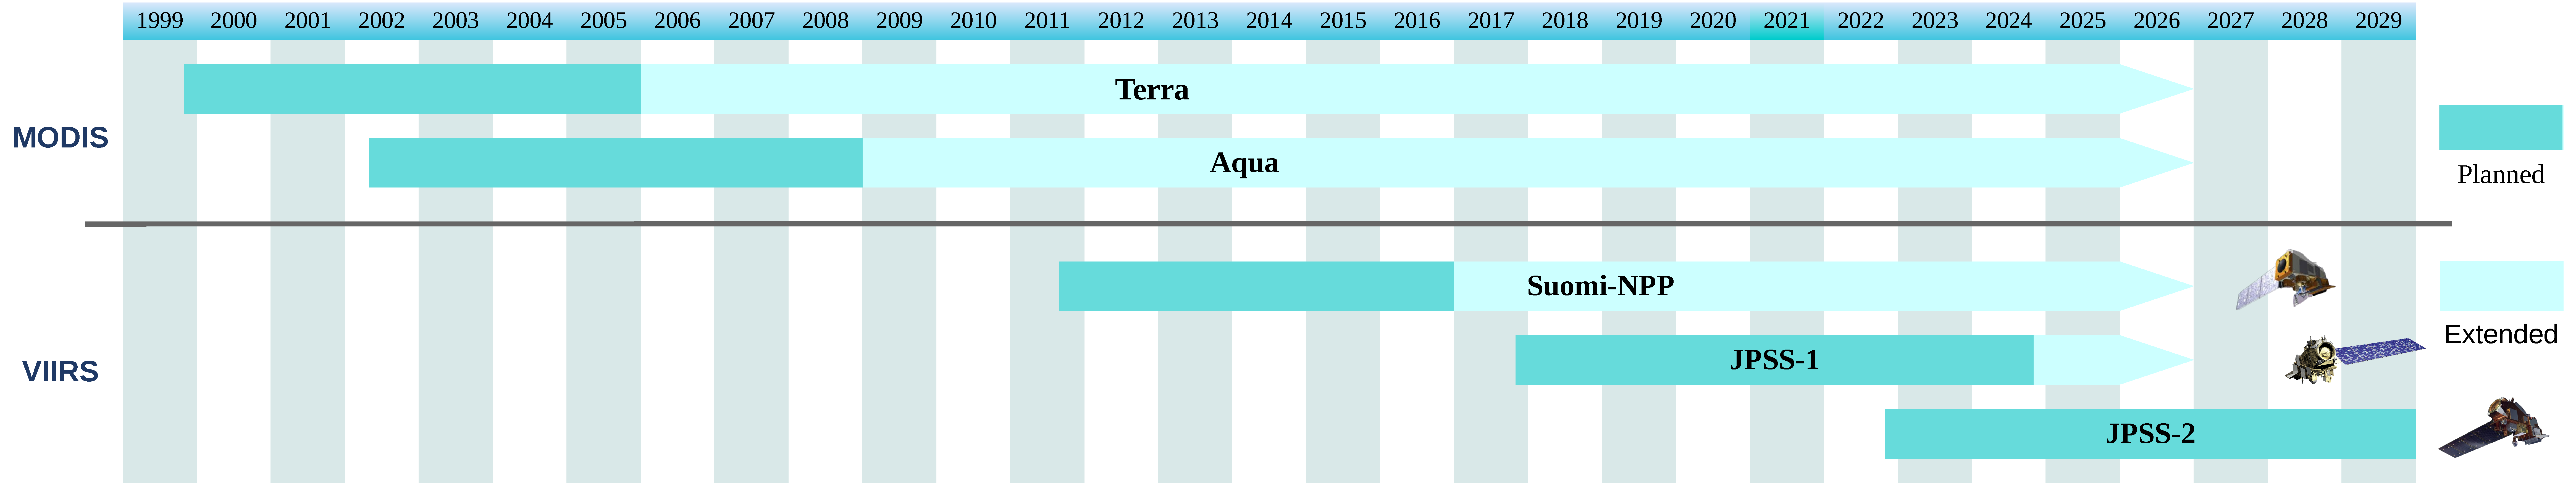
\includegraphics[scale=0.11]{./illustrations/fig01.pdf} 
\caption{Timeline of MODIS and VIIRS missions. VIIRS is a multi-spectral optical instrument onboard of 3 orbiting satellites operated by the United States National Oceanic and Atmospheric Administration (NOAA): Suomi NPP (Suomi National Polar-orbiting Partnership), launched in 2011, JPSS-1 (Joint Polar Satellite System) or NOAA-20 launched in 2017 and JPSS-2 (Joint Polar Satellite System) or NOAA-21 launched in 2022.}
\label{fig: timeline}
\end{figure*}


\section{Study area}
\label{subsec: study_area}

The study area corresponds to the operational coverage of the S2M snow modeling system and covers approximately 105 000~km² (Fig.~\ref{fig: aoi}). It comprises the main mountain ranges of continental France, i.e., from north to south: the Vosges, the Jura, the Northern Alps, the Massif Central, the Southern Alps, the Pyrenees, and Corsica. All massifs are located in France except the Spanish and Andorran part of the Pyrenees. To reduce the imbalance between snow-free and snow covered pixels in the analysis, we exclude areas below 900 meters of elevation. By applying this elevation threshold, we increase the fraction of snow covered pixels in the VNP10A1 dataset from 20\% to 31\% of valid (i.e., cloud-free) observations between the 1st of November and the 30th of June of the 2023/2024 winter season.

\begin{figure}
\centering
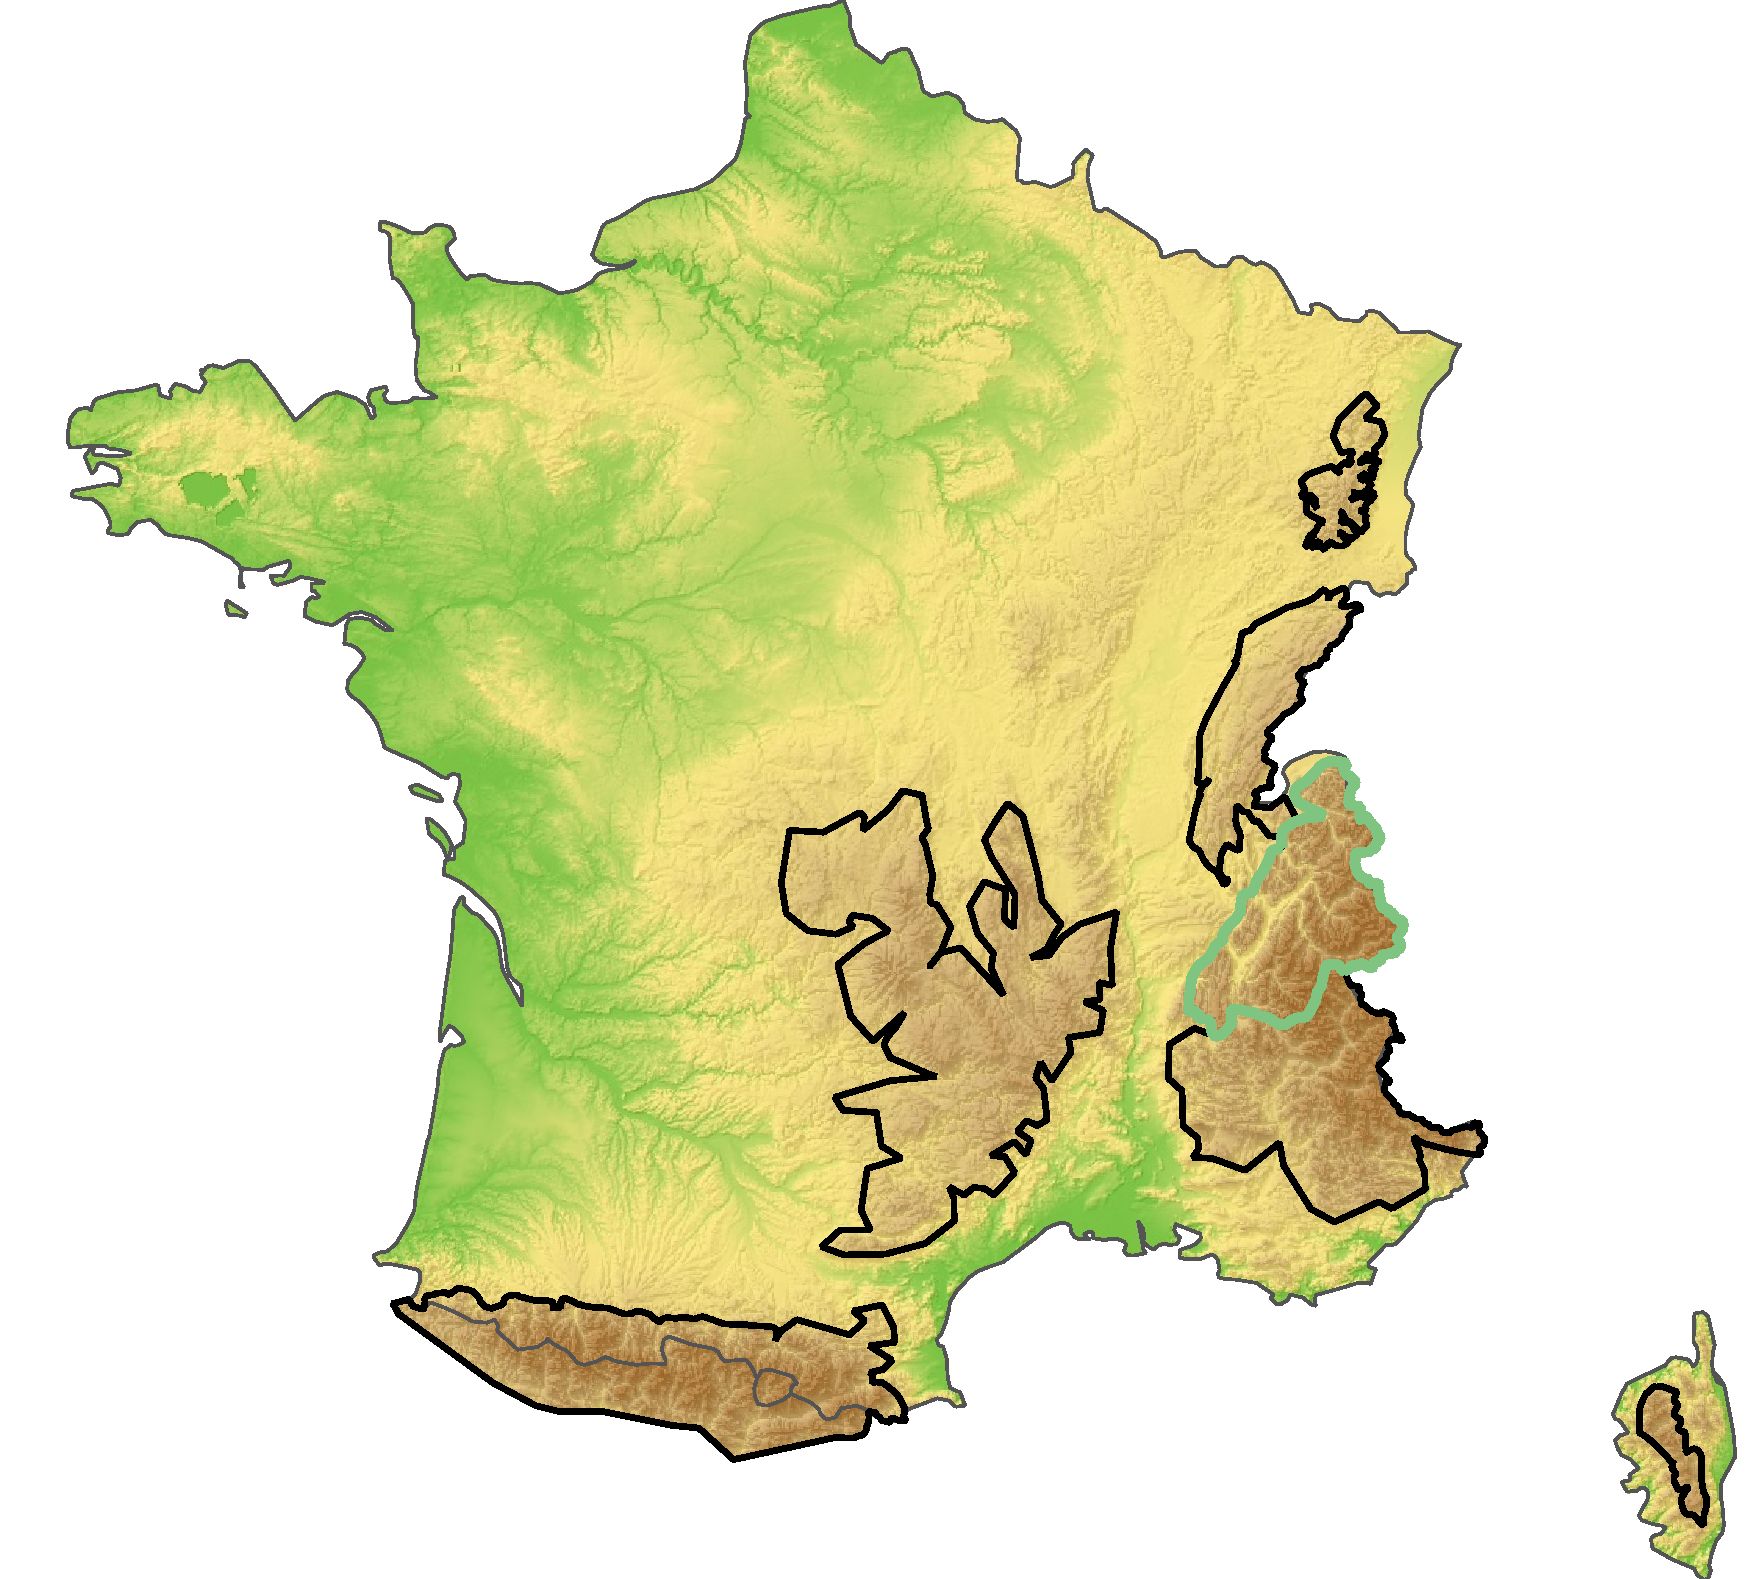
\includegraphics[scale=0.3]{./illustrations/fig02.pdf} 
\caption{The mountainous areas of France corresponding to our study area. The green outline defines the Northern Alps, shown in Fig.~\ref{fig: data_product_alpes}.} 
\label{fig: aoi}
\end{figure}


\section{Data}
\label{sec: data}
\begin{figure*}
\centering
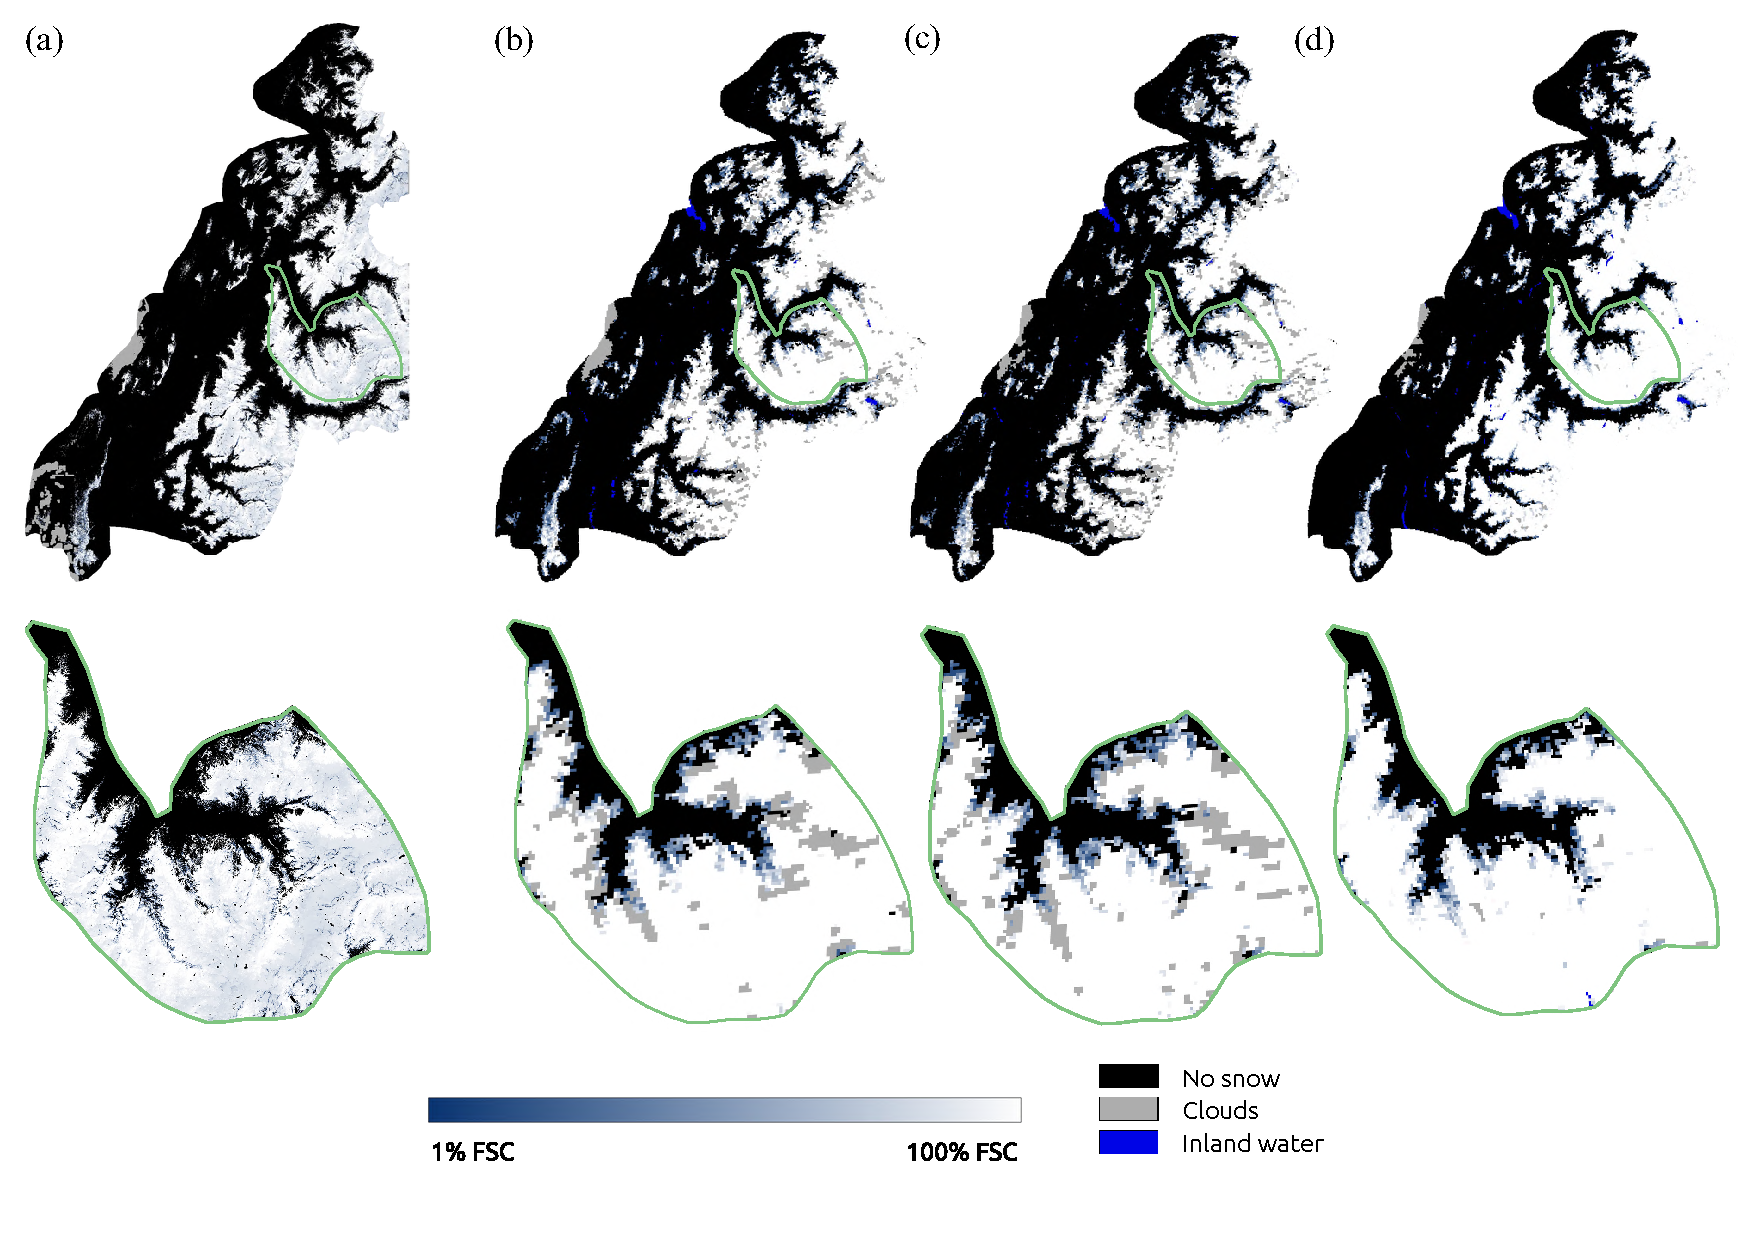
\includegraphics[scale=0.55]{./illustrations/fig03.pdf} 
\caption{Samples of the satellite products used in this work, 03/02/2024, on the Northern Alps (top) with zoom on the Vanoise massif (bottom) outlined in green. (a) Sentinel-2 Theia distribution; (b) VNP10A1 (c) VJ110A1  (d) MF-FSC-VNP-L3 (Météo-France FSC VIIRS SNPP daily composite) }
\label{fig: data_product_alpes}
\end{figure*}

\subsection{NASA V[NP\textbar J1]10A1 \DIFaddbegin \DIFadd{and M}[\DIFadd{O\textbar Y}]\DIFadd{D10A1}\DIFaddend }
\label{subsec: data_nasa}
The official distribution of VIIRS \DIFaddbegin \DIFadd{and MODIS }\DIFaddend snow cover products is provided by the National Snow and Ice Data Center (NSIDC) on behalf of NASA. 
The NSIDC DAAC VIIRS snow cover collection includes different product levels for both Suomi-NPP and JPSS-1 acquisitions,while products based on the JPSS-2 platform are not distributed at the time of writing \citep{riggs2023viirs}. 
V[NP\textbar J1]10A1 are level-3 daily composites from \DIFdelbegin \DIFdel{, }\DIFdelend respectively, SNPP and JPSS-1 observations\DIFdelbegin \DIFdel{, }\DIFdelend \DIFaddbegin \DIFadd{. M}[\DIFadd{O|Y}]\DIFadd{D10A1 is the equivalent product derived from MODIS sensor aboard Terra and Aqua platforms, respectively. All datasets are }\DIFaddend distributed on the MODIS sinusoidal grid. 
These products, similar to most optical operational snow cover products, are based on the NDSI, that is defined for VIIRS by Eq. \eqref{eq: ndsi}. 

\begin{equation}
    \mathrm{NDSI} = \frac{I1-I3}{I1+I3}
    \label{eq: ndsi}
\end{equation}

where $I1$ and $I3$ are the calibrated radiances (from V[NP\textbar J1]02IMG L1B 375~m IMG bands) centered, respectively, at 645~nm and 1635~nm. The processing is described in \DIFdelbegin \DIFdel{\mbox{%DIFAUXCMD
\citep{riggs2023viirs}}\hspace{0pt}%DIFAUXCMD
}\DIFdelend \DIFaddbegin \DIFadd{\mbox{%DIFAUXCMD
\citep{riggs2021MODISAquaSnow, riggs2025MODISTerraSnow}}\hspace{0pt}%DIFAUXCMD
}\DIFaddend . Snow detection is an NDSI-based algorithm that implements a cascade of spectral reflectance screens to limit omission and commission errors. %
\DIFdelbegin \DIFdel{This product does }\DIFdelend \DIFaddbegin \DIFadd{These products do }\DIFaddend not provide the snow cover fraction\DIFdelbegin \DIFdel{(fractional snow covered area), but only }\DIFdelend \DIFaddbegin \DIFadd{, but rather }\DIFaddend the NDSI of snow covered pixels (NDSI\_Snow\_Cover). This means that users wishing to extract snow cover fraction from VNP10 must apply a conversion function. \DIFdelbegin \DIFdel{As for the NSIDC distribution, we evaluate the VNP10A1 and VJ110A1 collections, which are the daily composites of the SNPP and JPSS-1 platform observations, respectively. }\DIFdelend The daily composition of multiple SNPP\DIFdelbegin \DIFdel{/}\DIFdelend \DIFaddbegin \DIFadd{, }\DIFaddend JPSS-1\DIFaddbegin \DIFadd{, Terra and Aqua }\DIFaddend acquisitions is performed using an algorithm  \DIFdelbegin \DIFdel{mainly }\DIFdelend based on the solar and view zenith angles \DIFdelbegin \DIFdel{\mbox{%DIFAUXCMD
\citep{riggs2023viirs}}\hspace{0pt}%DIFAUXCMD
}\DIFdelend \DIFaddbegin \DIFadd{\mbox{%DIFAUXCMD
\citep{riggs2023viirs, riggs2025MODISTerraSnow}}\hspace{0pt}%DIFAUXCMD
}\DIFaddend . We downloaded these data using earthaccess API \citep{barrett_2026_18435881}.

\subsection{Météo-France FSC VIIRS multi-platform daily composite}
\label{subsec: data_meteofrance}
We present, for the first time, the Météo-France FSC VIIRS multi-platform daily composite product. It is a daily composite of the SNPP, JPSS-1 and JPSS-2 VIIRS platform and covers continental France. It is produced by the
\textit{Centre de Météorologie Spatiale (CMS)}, the unit of Météo France responsible for delivering meteorological satellite images to the forecasters. It is released every day, only a few hours after the last day pass of a VIIRS platform over France. The format, a daily composite of the observations from the three VIIRS platforms, is chosen to synthesize daily information for mountain meteorological forecasters and to optimize daily assimilation into snowpack modeling system. The daily composition is performed using an algorithm based on the sensor zenith angle. In practice, for each ground cell, we choose the valid observation with the lowest zenith angle among all the VIIRS acquisitions, regardless of the platform that took it. The snow cover detection pipeline uses NOAA's VIIRS Sensor Data Records (SDR) TOA radiances as input. This differs from the NASA processing chain, which relies on NASA's L1B radiance distribution. The snow detection is an NDSI-based algorithm with a few screens to limit false detection. The algorithm and product format are detailed in Appendix \ref{app: mf_product}. 

\subsection{Sentinel-2 Theia snow products}
\label{subsec: data_sentinel2}
The reference products used in this study are sourced from the Sentinel-2 Theia Snow collection, a collection of 20~m resolution snow cover products generated from Sentinel-2 surface reflectances \citep{gascoin_theia_2019}. These products are available over most of Europe mountain ranges, and were extensively evaluated using in situ measurements and very-high resolution satellite images \citep{gascoin_theia_2019, barrou_dumont_brief_2021}. A recent benchmark study found that the Theia products exhibit the highest performance among high resolution snow products \citep{GARCIAGARCIA2026115131}. The current products include a minor upgrade with respect to the base algorithm that is described in \citep{gascoin_theia_2019}. An additional snow detection screen has been implemented to enhance the snow cover detection in steep shaded slopes based on the blue band. This upgrade is documented in the source code repository (release 1.8). An additional difference compared to the products described in \citep{gascoin_theia_2019} is that an estimate of the fractional snow cover (FSC) is provided for every snow pixel. This fraction is computed from the NDSI using an empirical relationship whose calibration is illustrated in \citep{gascoin_estimating_2020} in the Alps and the Pyrenees, and adjusted in forest areas to account for the obstruction of the ground by the tree canopy.
\begin{equation}
    \mathrm{FSC_{OG}} = \min(\frac{\mathrm{FSC_{TOC}}}{\mathrm{VGF}}, 1)
\end{equation}
\label{eq: fscog}
where $\mathrm{FSC_{OG}}$ and  $\mathrm{FSC_{TOC}}$ are, respectively, the on ground and the top-of-canopy fractional snow cover computed from the NDSI, and VGF is the viewable gap fraction computed from the 20~m resolution Copernicus tree cover density product (TCD):
\begin{equation}
    \mathrm{VGF} = 1 - \mathrm{TCD}
\end{equation}
\label{eq: vgf}
This latter modification was implemented for the Copernicus Land monitoring service and is described more extensively in \citep{hr-si_consortium_algorithm_2020}. 

\subsection{Auxiliary data}
\label{subsec: data_auxiliary}

Forest and topographic datasets are used to stratify the snow cover product error analysis (Sect.~\ref{subsec: obs_classes}). We use a forest mask from Corine 2018 \citep{corine2018}. The Digital Elevation Model (DEM) is obtained from LidarHD \citep{lidarhd} and Copernicus 30m \citep{copernicus_dem}. Per pixel zenith angle information is provided in the MF-FSC-V[MP\textbar NP\textbar J1\textbar J2]-L3 products (Appendix \ref{app: mf_product}). 

\section{Methods}
\label{sec: methods}

\subsection{Resampling to a common grid}
\label{subsec: meth_resampling} 

To perform per pixel comparison, we mosaic and regrid all datasets (VIIRS products and reference Sentinel-2) to a common WGS84/UTM grid with a spatial sampling of 375~m (VIIRS nominal spatial resolution). \DIFdelbegin \DIFdel{Any output grid pixel that is }\DIFdelend \DIFaddbegin \DIFadd{Although reprojecting both reference and target datasets may introduce an additional resampling error, this choice has concrete advantages as reprojecting any evaluated dataset (regardless of its original projection) is more straightforward than generating multiple reference datasets, one for each different VIIRS product projection. We verified (not shown) that the impact of this choice is the order of 0.5 - 1\% on the results. We treated the uncertainty linked to cloud masks by masking pixels that are }\DIFaddend even partially covered by a cloud in the \DIFdelbegin \DIFdel{input data is marked as cloudy. This causes the cloud masks to expand, but no assumptions are made about the surface conditions the clouds}\DIFdelend \DIFaddbegin \DIFadd{reference or target datasets}\DIFaddend . The same procedure is applied to other unusable classes like missing data, night, out-of-swath pixels, etc. Inland water classes are reprojected using nearest neighbor. The remaining FSC pixels between 0\% and 100\% are resampled via an average interpolation method. In such a scheme, the result is the average of the input grid pixels falling into the output grid pixel.

As mentioned in Sect. \ref{subsec: data_nasa}, the NASA products do not provide FSC, but rather the NDSI of snow covered pixels. Therefore, we convert NDSI to fractional snow cover using the "FRA6T" or "Universal relation" (Eq. \ref{eq: salomonson_appel}). Although this equation was fitted for MODIS data using Landsat as reference, it has also been applied to obtain FSC from VIIRS products \citep{stillinger_landsat_2023, jacques-hamilton_measurement_2025}\DIFaddbegin \DIFadd{.
}\DIFaddend \begin{equation}
    \mathrm{FSC} = -0.01 + 1.45 \, \mathrm{NDSI}
    \label{eq: salomonson_appel}
\end{equation}

The Météo-France FSC VIIRS  product is based on the same equation, what makes the comparison in terms of FSC fair between the two products and comparable to other similar evaluations \citep{masson_assessment_2018}. \DIFdelbegin %DIFDELCMD < 

%DIFDELCMD < %%%
\DIFdel{We aggregate Sentinel-2 FSC data to generate 375~m resolution reference snow maps expressed in snow cover fraction.  }\DIFdelend In \citep{gascoin_estimating_2020}, the authors used a sigmoid-shaped function of the NDSI to estimate $\mathrm{FSC_{TOC}}$ from Sentinel-2. This function was fit and tested using a spatially-limited dataset, and, therefore, its uncertainty is not well known in other regions. In particular, this function saturates near 90\% FSC even for high NDSI values, which could create a bias in high elevation areas that are presumably fully snow covered during winter (Fig.~\ref{fig: scatter}). To reduce the sensitivity of our reference Sentinel-2 FSC to this function, we perform a binarization of Sentinel-2 $\mathrm{FSC_{OG}}$ to snow/no-snow prior to aggregation to 375~m. This binarization is done using a threshold at 50\% $\mathrm{FSC_{OG}}$. We use the average interpolation function to resample the Sentinel-2 20~m binary products to the VIIRS 375~m resolution grid \citep{gdal}. As for the VIIRS products, output grid pixels that contain at least one invalid pixel in the input grid are set to invalid. 
We process \DIFdelbegin \DIFdel{every VIIRS }\DIFdelend \DIFaddbegin \DIFadd{each V}[\DIFadd{NP\textbar J1}]\DIFadd{10A1, MF-FSC-VNP-L3 }\DIFaddend and Sentinel-2 acquisition over our study area between the 1st November 2023 and the 30th June 2024. We obtain about 4 millions valid (cloud-free) match-ups between each one of our VIIRS datasets and the reference product derived from Sentinel-2. \DIFaddbegin \DIFadd{We repeat the same steps for MF-FSC-V}[\DIFadd{NP\textbar J1\textbar J2\textbar MP}]\DIFadd{-L3 and Sentinel-2 for the 2024/2025 season to assess our multi-platform composite against its individual platform components (Sec. \ref{subsec: data_meteofrance}). The same is done for VNP10A1 and M}[\DIFadd{O\textbar Y}]\DIFadd{D10A1 and Sentinel-2 for the comparison between VIIRS and MODIS, in season 2023/2024. The resampling UTM grid for this case study has a spatial sampling of 500~m to match the resolution of MODIS.
 }\DIFaddend 

\subsection{Analysis stratification} 
\label{subsec: obs_classes}

We resample the auxiliary datasets to the same WGS84/UTM grid as above, using the nearest neighbour interpolation (forest mask) and the Lanczos interpolation (DEM). Then, slope and aspect are computed using GDAL's gdaldem tools \citep{gdal}. We group the slope information in three classes representing low angles (0-10°), moderate angles (10°-30°), and steep terrain ($>$ 30°). The aspects are grouped in 8 bins centered in the cardinal and intercardinal directions: North (N), North-East (NE), East (E), South-East (SE), South (S), South-West (SW), West (W), North-West (NW). The V[NP\textbar J1]10A1 does not provide per pixel-wise data on the sensor viewing angle. However this information is included in the MF-FSC-VNP-L3, which allows us to analyze the performance of this product by bins of 15° view zenith angle. For each class of land cover, slope, etc., we compute the number of valid match-ups (i.e., the sample size). 

\subsection{Assessing multi-platform data fusion}
\label{subsec: meth_compo}

The operational Météo-France FSC VIIRS multi-platform daily composite is based on a fusion of VIIRS data onboard SNPP, JPSS-1 and JPSS-2 satellites (Fig.~\ref{fig: timeline}).  We compare the performance of the multi-platform composite to each individual daily composites (one per platform). Since JPSS-2 data have been available operationally only since May 2024, only in Météo-France computing infrastructure, we carry out this evaluation over the 2024/2025 winter season. We apply the same procedure illustrated in Section \ref{subsec: meth_resampling} on the same study area between 1st November 2024 and the 30th June 2025 and obtain a comparable number of valid match-ups (about 4 million) with the Sentinel-2 reference for each VIIRS product. 

\subsection{Snow cover area calculation}

We compute the snow cover area of the regridded products as the sum of the snow cover fraction pixels multiplied by the area of a pixel on the grid (375~m x 375~m). In the same manner, we compute the area covered by clouds. As the UTM projection is not equal area, this introduces a small error. The relative difference between the snow cover area computed in UTM projection and in geodesic coordinates (WGS84 ellipsoid) on a given date on the study area is on the order of  0.05\%. As we do not need precise area calculations, this allows us to use the area approximation in UTM coordinates. Since cloud cover (and consequently snow cover extent) is highly variable on a daily basis, the results in terms of snow cover area are presented using the monthly averaged daily area for each month.

\subsection{Binary scores}
\label{subsec: methods_binary}

We binarize the FSC values into "snow" and "no-snow" classes \DIFdelbegin \DIFdel{using a threshold of 50\%for both the reference and evaluation datasets}\DIFdelend \DIFaddbegin \DIFadd{by considering that all pixels with a valid FSC value (i.e. higher or equal to 1\%) are snow-covered}\DIFaddend . Then, we compute the confusion matrix between the reference and evaluation datasets, where true positive (TP) means that snow is correctly detected, true negative (TN) means that no-snow is correctly detected, false positive (FP) means that snow is detected whereas the reference indicates that no snow is present, and false negative (FN) means that no-snow was detected whereas the reference indicates that snow is present. \DIFdelbegin \DIFdel{We compute the accuracy, as it is a metric commonly used to quantify the performance of a detection algorithm (Eq. \ref{eq: accuracy}). However, this metric can be biased by the overrepresentation of no-snow cases (TNs represent approximately 80\% of the correspondences), which are less challenging to retrieve \mbox{%DIFAUXCMD
\citep{masson_assessment_2018}}\hspace{0pt}%DIFAUXCMD
. Thus, we also report the $F_1$ score (Eq. \ref{eq: f1_score}) \mbox{%DIFAUXCMD
\citep{rittger_evaluation_2021, zhang_comparative_2020}}\hspace{0pt}%DIFAUXCMD
.   
}\begin{displaymath}
    \DIFdel{\mathrm{Accuracy} = \frac{\mathrm{TP}+\mathrm{TN}}{\mathrm{TP}+\mathrm{TN}+\mathrm{FP}+\mathrm{FN}}
%DIFDELCMD < \label{eq: accuracy}%%%
}\end{displaymath}%DIFAUXCMD
%DIFDELCMD < 

%DIFDELCMD < %%%
\begin{displaymath}
    \DIFdel{\mathrm{F_1 ~ score} = \frac{2~\mathrm{TP}}{2~\mathrm{TP}+\mathrm{FP}+\mathrm{FN}}
\label{eq: f1_score}
}\end{displaymath}%DIFAUXCMD
%DIFDELCMD < 

%DIFDELCMD < %%%
\DIFdel{In addition, we complement the analysis by computing }\DIFdelend \DIFaddbegin \DIFadd{From the confusion matrix, we compute }\DIFaddend the commission (Eq. \ref{eq: comm_err}) and omission (Eq. \ref{eq: om_err}) errors. These metrics can be seen, respectively, as the probability of false snow detection and the product's tendency to underestimate snow presence \citep{schwaizer2020SnowCoverExtentb}\DIFaddbegin \DIFadd{.
}\DIFaddend \begin{equation}
    \mathrm{Commission ~ error} = \frac{\mathrm{FP}}{\mathrm{FP}+\mathrm{FN}}
\label{eq: comm_err}
\end{equation}


\begin{equation}
    \mathrm{Omission ~ error} = \frac{\mathrm{FN}}{\mathrm{FP}+\mathrm{TN}}
\label{eq: om_err}
\end{equation}

\DIFaddbegin \DIFadd{The binary snow detection performance is summarized by the $\mathrm{F_1}$ score (Eq. \ref{eq: f1_score}) \mbox{%DIFAUXCMD
\citep{rittger_evaluation_2021, zhang_comparative_2020}}\hspace{0pt}%DIFAUXCMD
, which is the harmonic mean of omission and commission.
}\begin{equation}
    \DIFadd{\mathrm{F_1 ~ score} = \frac{2~\mathrm{TP}}{2~\mathrm{TP}+\mathrm{FP}+\mathrm{FN}}
\label{eq: f1_score}
}\end{equation}





\DIFaddend \subsection{FSC error distribution}
\label{subsec: methods_distribution}

We compute the bias and Root Mean Square Error (RMSE) of all $ N $ valid pixel correspondences between the reference and the VIIRS \DIFaddbegin \DIFadd{or MODIS }\DIFaddend observations (Eq. \ref{eq: biais} and \ref{eq: rmse}). We use $y$ to refer to the VIIRS \DIFaddbegin \DIFadd{or MODIS }\DIFaddend FSC and $y^*$ to refer to the reference Sentinel-2 FSC.


\begin{equation}
 \mathrm{Bias} = \frac{1}{N} \sum_{i=0}^{N} (y_i - y^*_i)
\label{eq: biais}
\end{equation}


\begin{equation}
 \mathrm{RMSE} = \sqrt{\frac{1}{N}\sum_{i=0}^{N} (y_i - y^*_i)^2}
 \label{eq: rmse}
\end{equation}


\section{Results}
\label{sec: results}

\subsection{General performance}
\label{subsec: res_global}


\begin{table*}[t]
    \caption{Aggregated scores for VNP10A1, VJ110A1 and MF-FSC-VNP-L3 on our benchmark. Besides binary and error distribution scores, we report the total number of valid match-ups considered per product and the percentage of snow covered pixels among them.}
    \DIFdelbeginFL %DIFDELCMD < \label{tab: tab03}
%DIFDELCMD <     \begin{tabular}{l|R{2cm}R{2cm}|R{1.3cm} R{1.3cm} R{1.3cm}R{1.3cm}|R{1.3cm}R{1.3cm}}
%DIFDELCMD <         %%%
\DIFdelendFL \DIFaddbeginFL \label{tab: tab04}
    \begin{tabular}{l|R{2cm}R{2cm}|R{1.3cm} R{1.3cm}R{1.3cm}|R{1.3cm}R{1.3cm}}
        \DIFaddendFL \hline
        Product & N Valid Match-ups &\% Snow Cover & \DIFdelbeginFL \DIFdelFL{Accuracy }%DIFDELCMD < & %%%
\DIFdelendFL $\mathrm{F_1}$ score & \raggedleft Commission Error & Omission Error & Bias [\%] & RMSE [\%] \\
        \hline
        VNP10A1			& \DIFdelbeginFL \DIFdelFL{4.33}\DIFdelendFL \DIFaddbeginFL \DIFaddFL{4.48}\DIFaddendFL e+06 & \DIFdelbeginFL \DIFdelFL{17.7 }\DIFdelendFL \DIFaddbeginFL \DIFaddFL{26.0	}\DIFaddendFL & \DIFdelbeginFL %DIFDELCMD < \bfseries %%%
\DIFdelFL{0.98 }\DIFdelendFL \DIFaddbeginFL \DIFaddFL{0.91 				}\DIFaddendFL & \DIFdelbeginFL %DIFDELCMD < \bfseries %%%
\DIFdelFL{0.93 }\DIFdelendFL \DIFaddbeginFL \DIFaddFL{0.03 				}\DIFaddendFL & \bfseries \DIFdelbeginFL \DIFdelFL{0.01 }%DIFDELCMD < & %%%
\DIFdelFL{0.07 }\DIFdelendFL \DIFaddbeginFL \DIFaddFL{0.10 	}\DIFaddendFL & \DIFdelbeginFL %DIFDELCMD < \bfseries %%%
\DIFdelFL{0.07 }\DIFdelendFL \DIFaddbeginFL \DIFaddFL{0.42			}\DIFaddendFL & \bfseries \DIFdelbeginFL \DIFdelFL{9.82 }\DIFdelendFL \DIFaddbeginFL \DIFaddFL{10.09 }\DIFaddendFL \\
        VJ110A1 		& 4.45e+06 & \DIFdelbeginFL \DIFdelFL{18.6 }%DIFDELCMD < & %%%
\DIFdelFL{0.97 }\DIFdelendFL \DIFaddbeginFL \DIFaddFL{25.2 	}\DIFaddendFL & \DIFdelbeginFL \DIFdelFL{0.93 }\DIFdelendFL \DIFaddbeginFL \DIFaddFL{0.89 				}\DIFaddendFL & \DIFdelbeginFL \DIFdelFL{0.02 }\DIFdelendFL \DIFaddbeginFL \DIFaddFL{0.04 				}\DIFaddendFL & \bfseries \DIFdelbeginFL \DIFdelFL{0.07 }\DIFdelendFL \DIFaddbeginFL \DIFaddFL{0.10 	}\DIFaddendFL & \DIFdelbeginFL \DIFdelFL{0.35 }\DIFdelendFL \DIFaddbeginFL \DIFaddFL{0.81 			}\DIFaddendFL & \DIFdelbeginFL \DIFdelFL{10.81 }\DIFdelendFL \DIFaddbeginFL \DIFaddFL{10.88 }\DIFaddendFL \\
        MF-FSC-VNP-L3 	& 4.89e+06 & \DIFdelbeginFL \DIFdelFL{22.5 }%DIFDELCMD < & %%%
\DIFdelFL{0.96 }\DIFdelendFL \DIFaddbeginFL \DIFaddFL{30.1 	}\DIFaddendFL & \DIFaddbeginFL \bfseries \DIFaddendFL 0.92 	& \DIFaddbeginFL \bfseries \DIFaddendFL 0.02 	& \DIFdelbeginFL \DIFdelFL{0.10 }\DIFdelendFL \DIFaddbeginFL \DIFaddFL{0.11 				}\DIFaddendFL &\DIFdelbeginFL \DIFdelFL{-0.96 }\DIFdelendFL \DIFaddbeginFL \bfseries \DIFaddFL{0.41	}\DIFaddendFL & \DIFdelbeginFL \DIFdelFL{14.79 }\DIFdelendFL \DIFaddbeginFL \DIFaddFL{14.73 }\DIFaddendFL \\
        \hline
    \end{tabular}
\end{table*}


Table \DIFdelbegin \DIFdel{\ref{tab: tab03} }\DIFdelend \DIFaddbegin \DIFadd{\ref{tab: tab04} }\DIFaddend summarizes the performance of the three products. \DIFaddbegin \DIFadd{We observe that the number of valid match-ups (more than 4 million) and the snow cover percentage (between 25\% and 30\%) are comparable for the three products and make the comparison fair. }\DIFaddend MF-FSC-VNP-L3 has \DIFaddbegin \DIFadd{roughly }\DIFaddend 10\% more valid match-ups \DIFaddbegin \DIFadd{and 5\% more snow-covered area among the correspandences}\DIFaddend , suggesting that Météo-France cloud mask algorithm is less conservative than \DIFdelbegin \DIFdel{the NASAcloud mask algorithm}\DIFdelend \DIFaddbegin \DIFadd{NASA's}\DIFaddend . The snow detection performance of the three products are similar. MF-FSC-VNP-L3 \DIFdelbegin \DIFdel{has fewer false positive (commission error 0.02) at the cost of }\DIFdelend \DIFaddbegin \DIFadd{achieves the best  $\mathrm{F_1}$ score of 92\%, while it is of 91\% for VNP10A1 and 89\% for VJ110A1. MF-FSC-VNP-L3 has }\DIFaddend a higher omission error (\DIFaddbegin \DIFadd{0.11 compared to }\DIFaddend 0.10 \DIFdelbegin \DIFdel{). This is consistent with the slightly more negative bias (-1\% ) than that obtained from the NASA products(}\DIFdelend \DIFaddbegin \DIFadd{for V}[\DIFadd{NP\textbar J1}]\DIFadd{10A1) and lower commission error (0.02 compared to 0.03 for VNP10A1 and 0.04 for VJ110A1). The bias is between }\DIFaddend 0 \DIFdelbegin \DIFdel{\%). The dispersion of the residuals is also }\DIFdelend \DIFaddbegin \DIFadd{and 1\% for the three products. The RMSE is significantly }\DIFaddend higher for MF-FSC-VNP-L3, with an RMSE of \DIFaddbegin \DIFadd{almost }\DIFaddend 15\%, while \DIFdelbegin \DIFdel{VNP10A1 and VJ110A1 have an RMSE of }\DIFdelend \DIFaddbegin \DIFadd{it is of roughly }\DIFaddend 10 and 11\% \DIFaddbegin \DIFadd{for VNP10A1 and VJ110A1}\DIFaddend , respectively. 
\DIFdelbegin \DIFdel{Finally, we observe that the number of valid match-ups (more than 4 million) and the snow cover percentage (about 20\%) are comparable for the three products. 
}\DIFdelend 


\subsection{Performance detailed analysis}
\label{subsec: res_charcaterization}

\begin{figure*}
\centering
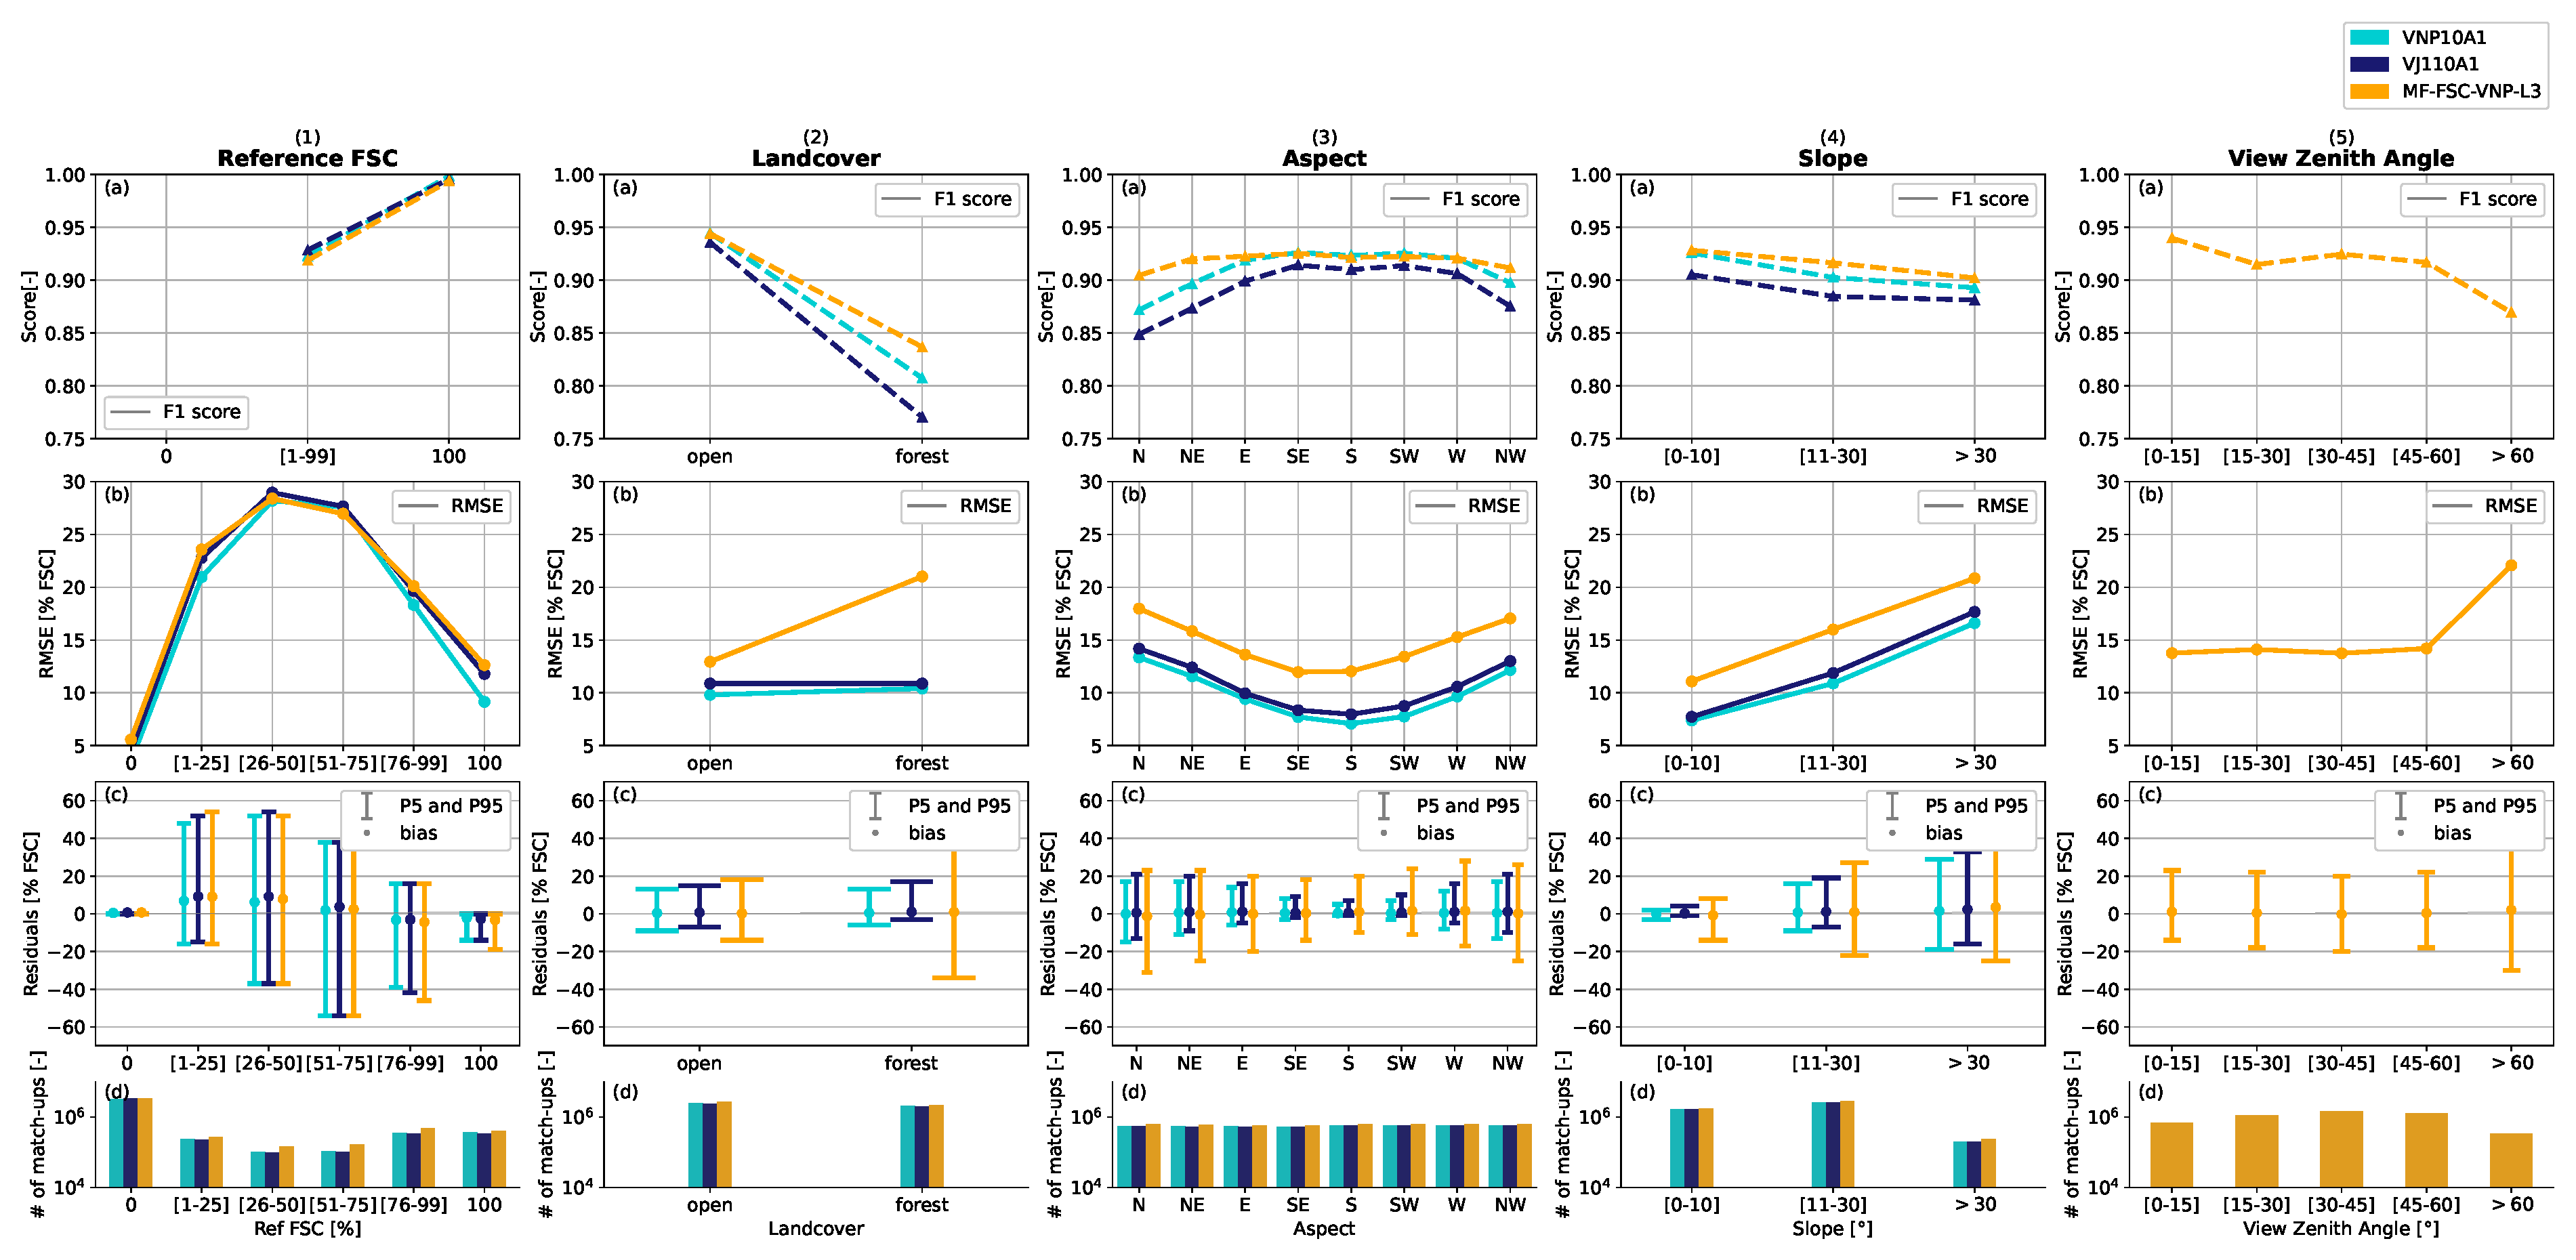
\includegraphics[scale=0.28]{./illustrations/fig04.eps} 
\caption{Performance metrics of VIIRS snow cover products as a function of the following factors: (1) reference (Sentinel-2) FSC, (2) land cover (forest vs bare soil), (3) aspect, (4) slope, (5) view zenith angle. The metrics presented are: (a) \DIFdelbeginFL \DIFdelFL{accuracy and }\DIFdelendFL $\mathrm{F_1}$ score, (b) RMSE, (c) error bars showing the 5th and 95th percentile range and bias, (d) number of valid match-ups. The satellite products considered are: MF-FSC-VNP-L3 (orange), VNP10A1 (light blue), and VJ110A1 (blue). }
\label{fig: synthesis}
\end{figure*}


\DIFdelbegin \DIFdel{The accuracy ranges from 94 to 98\% for most observation classes, while the $\mathrm{F_1}$ score ranges from 78\% to 95\% (}\DIFdelend Fig.~\ref{fig: synthesis}, panels (1-4)a \DIFdelbegin \DIFdel{)}\DIFdelend \DIFaddbegin \DIFadd{shows that the $\mathrm{F_1}$ score ranges from 76\% to 99\% under different conidition}\DIFaddend . We find an excellent performance \DIFdelbegin \DIFdel{with }\DIFdelend \DIFaddbegin \DIFadd{for }\DIFaddend pixels that are either fully \DIFdelbegin \DIFdel{snow-free (0\%) or fully }\DIFdelend snow-covered\DIFdelbegin \DIFdel{(100\%)}\DIFdelend \DIFaddbegin \DIFadd{, while the $\mathrm{F_1}$ score is not defined for pixels that are fully snow-free}\DIFaddend . The classification performance decreases when considering mixed pixels (1–99\%). The \DIFdelbegin \DIFdel{worst }\DIFdelend performance in terms of $\mathrm{F_1}$ score is \DIFdelbegin \DIFdel{found in forested }\DIFdelend \DIFaddbegin \DIFadd{systematically worse in forested than open }\DIFaddend areas for the three products (\DIFdelbegin \DIFdel{panel }\DIFdelend \DIFaddbegin \DIFadd{panela }\DIFaddend 2a). We also find that the performance of VIIRS products depends on the slope aspect (\DIFdelbegin \DIFdel{maximal on southern slopes and }\DIFdelend minimal on northern \DIFdelbegin \DIFdel{slopes}\DIFdelend \DIFaddbegin \DIFadd{aspects and similar elsewhere}\DIFaddend , panel 3a) and decreases with the terrain slope (panel 4a). The analysis further shows a limited impact of the sensor zenith angle on the MF-FSC-VNP-L3 \DIFdelbegin \DIFdel{product accuracy}\DIFdelend \DIFaddbegin \DIFadd{snow detection}\DIFaddend , except above 60°, where the performance strongly decreases (panel 5a). Table \DIFdelbegin \DIFdel{\ref{tab: tab04} reports accuracy, }\DIFdelend \DIFaddbegin \DIFadd{\ref{tab: tab05} reports }\DIFaddend $\mathrm{F_1}$ score, commission and omission errors of the VNP10A1 products for a combination of aspect and forest cover. \DIFdelbegin \DIFdel{Commission errors are substantially higher for mixed pixels because threshold-induced discrepancies matter when only 1–99\% reference snow cover pixels are considered, but become negligible when true positives and true negatives dominate}\DIFdelend \DIFaddbegin \DIFadd{The snow detection performance does not decrease in mixed pixels in terms of $\mathrm{F_1}$ score, while in the forest is systematically worse than in the corresponding open areas. In open areas, we find the same scores in North and South slopes. The worse $\mathrm{F_1}$ score (75\%) is found in forested, north slopes, where we find also the highest comission error}\DIFaddend . Omission errors are generally higher than commission errors, indicating that the reference (Sentinel-2) identifies substantially more snow, especially under forest canopy, where omission \DIFdelbegin \DIFdel{can reach 0.2–0.3. A similar increase is observed for north-facing slopes}\DIFdelend \DIFaddbegin \DIFadd{error can reach 0.23}\DIFaddend .

The number of valid match-ups shown in panels (1-5)d of Figure \ref{fig: synthesis} and in the fourth column of Table \DIFdelbegin \DIFdel{\ref{tab: tab04} }\DIFdelend \DIFaddbegin \DIFadd{\ref{tab: tab05} }\DIFaddend shows that the number of valid correspondences ranges is at least in the order of $10^4$ and at most of $10^6$ for the considered observation classes. The percentage of snow covered pixels (fifth column of Table~\DIFdelbegin \DIFdel{\ref{tab: tab04}}\DIFdelend \DIFaddbegin \DIFadd{\ref{tab: tab05}}\DIFaddend ) is variable and can be less then 10\% for some categories. For example, in forested areas for non mixed pixels, only \DIFdelbegin \DIFdel{3 }\DIFdelend \DIFaddbegin \DIFadd{8 }\DIFaddend (South) to \DIFdelbegin \DIFdel{7}\DIFdelend \DIFaddbegin \DIFadd{18}\DIFaddend \% (North) of the correspondences are snow covered.


\begin{table*}[t]
    \caption{VNP10A1 error distribution for some relevant combination of observation classes in terms of snow detection. We also report the number of valid match-ups for each row and the percentage of snow cover as the ratio between the number of pixels with FSC $>$ 50\% and the total number of pixels of the reference.}
    \DIFdelbeginFL %DIFDELCMD < \label{tab: tab04}
%DIFDELCMD <     \begin{tabular}{p{1.1cm}|p{1.1cm}p{0.9cm}|R{1.4cm}R{1.3cm}|R{1.2cm}R{1.2cm}R{1.3cm}R{1.3cm}|R{1.1cm}R{1.3cm}}
%DIFDELCMD <         %%%
\DIFdelendFL \DIFaddbeginFL \label{tab: tab05}
    \begin{tabular}{p{1.1cm}|p{1.1cm}p{0.9cm}|R{1.5cm}R{1.1cm}|R{1.1cm}R{1.4cm}R{1.4cm}|R{1.2cm}R{1.4cm}}
        \DIFaddendFL \hline
        Ref. FSC & Landcover & Aspect &N valid match-ups&\% Snow Cover  & \DIFdelbeginFL \DIFdelFL{Accuracy }%DIFDELCMD < & %%%
\DIFdelendFL $\mathrm{F_1}$ score & Commission Error & Omission Error & Bias [\%] & RMSE [\%] \\
        \hline
        1-99\% 	& Forest	& N	& \DIFdelbeginFL \DIFdelFL{4.57}\DIFdelendFL \DIFaddbeginFL \DIFaddFL{4.99}\DIFaddendFL e+04	& \DIFdelbeginFL \DIFdelFL{38.4 }%DIFDELCMD < & %%%
\DIFdelFL{0.76 }\DIFdelendFL \DIFaddbeginFL \DIFaddFL{100	}\DIFaddendFL & \DIFdelbeginFL \DIFdelFL{0.69 }\DIFdelendFL \DIFaddbeginFL \DIFaddFL{0.87 	}\DIFaddendFL & \DIFdelbeginFL \DIFdelFL{0.19 }\DIFdelendFL \DIFaddbeginFL \DIFaddFL{- 	}\DIFaddendFL & \DIFdelbeginFL \DIFdelFL{0.31 }\DIFdelendFL \DIFaddbeginFL \DIFaddFL{0.23 }\DIFaddendFL & \DIFdelbeginFL \DIFdelFL{-2.95 }\DIFdelendFL \DIFaddbeginFL \DIFaddFL{-1.38	}\DIFaddendFL & \DIFdelbeginFL \DIFdelFL{30.10 }\DIFdelendFL \DIFaddbeginFL \DIFaddFL{29.72 }\DIFaddendFL \\
        1-99\% 	& Forest 	& S & \DIFdelbeginFL \DIFdelFL{1.14}\DIFdelendFL \DIFaddbeginFL \DIFaddFL{1.28}\DIFaddendFL e+04	& \DIFdelbeginFL \DIFdelFL{40.5 }%DIFDELCMD < & %%%
\DIFdelFL{0.84 }\DIFdelendFL \DIFaddbeginFL \DIFaddFL{100 	}\DIFaddendFL & \DIFdelbeginFL \DIFdelFL{0.80 }\DIFdelendFL \DIFaddbeginFL \DIFaddFL{0.88 	}\DIFaddendFL & \DIFdelbeginFL \DIFdelFL{0.12 }\DIFdelendFL \DIFaddbeginFL \DIFaddFL{- 	}\DIFaddendFL & 0.21 & \DIFdelbeginFL \DIFdelFL{-3.06 }\DIFdelendFL \DIFaddbeginFL \DIFaddFL{-1.86 	}\DIFaddendFL & \DIFdelbeginFL \DIFdelFL{22.58 }\DIFdelendFL \DIFaddbeginFL \DIFaddFL{22.97 }\DIFaddendFL \\
        1-99\% 	& Open		& N & \DIFdelbeginFL \DIFdelFL{5.82}\DIFdelendFL \DIFaddbeginFL \DIFaddFL{6.58}\DIFaddendFL e+\DIFdelbeginFL \DIFdelFL{05 }\DIFdelendFL \DIFaddbeginFL \DIFaddFL{04	}\DIFaddendFL & \DIFdelbeginFL \DIFdelFL{65.7 }\DIFdelendFL \DIFaddbeginFL \DIFaddFL{100 	}\DIFaddendFL & \DIFdelbeginFL \DIFdelFL{0.86 }\DIFdelendFL \DIFaddbeginFL \DIFaddFL{0.93 	}\DIFaddendFL & \DIFdelbeginFL \DIFdelFL{0.89 }\DIFdelendFL \DIFaddbeginFL \DIFaddFL{- 	}\DIFaddendFL & 0.13 & \DIFdelbeginFL \DIFdelFL{0.15 }%DIFDELCMD < & %%%
\DIFdelFL{-4.17 }\DIFdelendFL \DIFaddbeginFL \DIFaddFL{-1.74 	}\DIFaddendFL & \DIFdelbeginFL \DIFdelFL{23.87 }\DIFdelendFL \DIFaddbeginFL \DIFaddFL{23.06 }\DIFaddendFL \\
        1-99\% 	& Open 		& S & \DIFdelbeginFL \DIFdelFL{5.08}\DIFdelendFL \DIFaddbeginFL \DIFaddFL{5.76}\DIFaddendFL e+04 	& \DIFdelbeginFL \DIFdelFL{61.3 }%DIFDELCMD < & %%%
\DIFdelFL{0.91 }\DIFdelendFL \DIFaddbeginFL \DIFaddFL{100 	}\DIFaddendFL & 0.93 	& \DIFdelbeginFL \DIFdelFL{0.13 }\DIFdelendFL \DIFaddbeginFL \DIFaddFL{- 	}\DIFaddendFL & \DIFdelbeginFL \DIFdelFL{0.06 }\DIFdelendFL \DIFaddbeginFL \DIFaddFL{0.13 }\DIFaddendFL & \DIFdelbeginFL \DIFdelFL{1.14 }\DIFdelendFL \DIFaddbeginFL \DIFaddFL{3.31 	}\DIFaddendFL & \DIFdelbeginFL \DIFdelFL{17.71 }\DIFdelendFL \DIFaddbeginFL \DIFaddFL{18.01 }\DIFaddendFL \\
        0-100\% & Forest 	& N & \DIFdelbeginFL \DIFdelFL{3.07}\DIFdelendFL \DIFaddbeginFL \DIFaddFL{3.18}\DIFaddendFL e+05 	& \DIFdelbeginFL \DIFdelFL{7.3 }%DIFDELCMD < & %%%
\DIFdelFL{0.96 }\DIFdelendFL \DIFaddbeginFL \DIFaddFL{17.9 	}\DIFaddendFL & \DIFdelbeginFL \DIFdelFL{0.73 }\DIFdelendFL \DIFaddbeginFL \DIFaddFL{0.75 	}\DIFaddendFL & \DIFdelbeginFL \DIFdelFL{0.02 }\DIFdelendFL \DIFaddbeginFL \DIFaddFL{0.07 	}\DIFaddendFL & \DIFdelbeginFL \DIFdelFL{0.27 }\DIFdelendFL \DIFaddbeginFL \DIFaddFL{0.20 }\DIFaddendFL & \DIFdelbeginFL \DIFdelFL{0.23 }\DIFdelendFL \DIFaddbeginFL \DIFaddFL{0.42 	}\DIFaddendFL & \DIFdelbeginFL \DIFdelFL{13.36 }\DIFdelendFL \DIFaddbeginFL \DIFaddFL{13.63 }\DIFaddendFL \\
        0-100\% & Forest 	& S & \DIFdelbeginFL \DIFdelFL{1.95}\DIFdelendFL \DIFaddbeginFL \DIFaddFL{2.02}\DIFaddendFL e+05 	& \DIFdelbeginFL \DIFdelFL{3.1 }%DIFDELCMD < & \bfseries %%%
\DIFdelFL{0.99 }\DIFdelendFL \DIFaddbeginFL \DIFaddFL{7.9 	}\DIFaddendFL & \DIFdelbeginFL \DIFdelFL{0.84 }\DIFdelendFL \DIFaddbeginFL \DIFaddFL{0.85	}\DIFaddendFL & \DIFdelbeginFL %DIFDELCMD < \bfseries %%%
\DIFdelFL{0.00 }\DIFdelendFL \DIFaddbeginFL \DIFaddFL{0.01 	}\DIFaddendFL & 0.17 & \DIFdelbeginFL %DIFDELCMD < \bfseries %%%
\DIFdelFL{-0.15 }\DIFdelendFL \DIFaddbeginFL \DIFaddFL{-0.13 	}\DIFaddendFL & \DIFdelbeginFL %DIFDELCMD < \bfseries %%%
\DIFdelFL{6.02 }\DIFdelendFL \DIFaddbeginFL \DIFaddFL{6.42 }\DIFaddendFL \\
        0-100\% & Open 		& N & \DIFdelbeginFL \DIFdelFL{2.36}\DIFdelendFL \DIFaddbeginFL \DIFaddFL{2.44}\DIFaddendFL e+05 	& \DIFdelbeginFL \DIFdelFL{35.7 }%DIFDELCMD < & %%%
\DIFdelFL{0.96 }\DIFdelendFL \DIFaddbeginFL \DIFaddFL{44.7 	}\DIFaddendFL & \DIFdelbeginFL \DIFdelFL{0.95 }\DIFdelendFL \DIFaddbeginFL \DIFaddFL{0.94 	}\DIFaddendFL & \DIFdelbeginFL \DIFdelFL{0.02 }\DIFdelendFL \DIFaddbeginFL \DIFaddFL{0.03 	}\DIFaddendFL & \DIFdelbeginFL \DIFdelFL{0.07 }\DIFdelendFL \DIFaddbeginFL \DIFaddFL{0.08 }\DIFaddendFL & \DIFdelbeginFL \DIFdelFL{-1.23 }\DIFdelendFL \DIFaddbeginFL \DIFaddFL{-0.64 	}\DIFaddendFL & \DIFdelbeginFL \DIFdelFL{12.86 }\DIFdelendFL \DIFaddbeginFL \DIFaddFL{13.00 }\DIFaddendFL \\
        0-100\% & Open 		& S & \DIFdelbeginFL \DIFdelFL{3.59}\DIFdelendFL \DIFaddbeginFL \DIFaddFL{3.69}\DIFaddendFL e+05 	& \DIFdelbeginFL \DIFdelFL{17.7 }%DIFDELCMD < & %%%
\DIFdelFL{0.99 }\DIFdelendFL \DIFaddbeginFL \DIFaddFL{23.6 	}\DIFaddendFL & \DIFdelbeginFL %DIFDELCMD < \bfseries %%%
\DIFdelFL{0.96 }\DIFdelendFL \DIFaddbeginFL \DIFaddFL{0.94 	}\DIFaddendFL & \DIFdelbeginFL \DIFdelFL{0.00 }\DIFdelendFL \DIFaddbeginFL \DIFaddFL{0.01 	}\DIFaddendFL & \DIFdelbeginFL %DIFDELCMD < \bfseries %%%
\DIFdelFL{0.03 }\DIFdelendFL \DIFaddbeginFL \DIFaddFL{0.08 }\DIFaddendFL &  \DIFdelbeginFL \DIFdelFL{0.18 }\DIFdelendFL \DIFaddbeginFL \DIFaddFL{0.55 	}\DIFaddendFL & \DIFdelbeginFL \DIFdelFL{6.95 }\DIFdelendFL \DIFaddbeginFL \DIFaddFL{7.43 }\DIFaddendFL \\
        \hline
    \end{tabular}
\end{table*}

Figure \ref{fig: synthesis} shows how the RMSE varies across the observation classes in panels 1–5b. Excluding mixed pixels (panel 1b), RMSE ranges from 7–16\% for VNP10A1, 8–17\% for VJ110A1, and 12–21\% for MF-FSC-VNP-L3. Panel 1b highlights that mixed pixels require particular attention, as they yield the highest errors, with RMSE reaching almost 30\% for FSC values between 25\% and 75\%. The NASA products appear relatively robust to forest canopy effects, whereas the MF product shows an increase in RMSE from 13\% on bare soil to 21\% in forested areas (panel 2b). The influence of topography (panels 2c–2d) follows similar patterns for all products and \DIFdelbegin \DIFdel{is consistent with the  trends observed }\DIFdelend \DIFaddbegin \DIFadd{the  and is more accentuated than }\DIFaddend for the binary metrics. Likewise, the performance decreases for view zenith angles above 60° (panel 2e).

Panels (1–5)c present the 5th–95th percentile range of the residuals, along with the mean error (circle). Excluding mixed pixels, all three products exhibit biases close to zero and largely symmetric error distributions. Overall, the two NASA products show consistent behavior, with VJ110A1 displaying slightly higher FSC values, while MF-FSC-VNP-L3 generally shows a wider error spread across most observation classes. Because most distributions are centered and symmetric, the patterns observed in panels (1–5)b for the RMSE are reflected here as well. Notable exceptions include panel \DIFdelbegin \DIFdel{3b}\DIFdelend \DIFaddbegin \DIFadd{3c}\DIFaddend , where NASA products show a low positive bias, indicating more snow cover in forests relative to the reference, and panels 3c and 3d, which show that \DIFdelbegin \DIFdel{Météo-France FSC L3 }\DIFdelend \DIFaddbegin \DIFadd{MF-FSC-VNP-L3 }\DIFaddend tends to underestimate snow cover on north-facing and low-slope ($<$10°) terrain.


Table \DIFdelbegin \DIFdel{\ref{tab: tab04} }\DIFdelend \DIFaddbegin \DIFadd{\ref{tab: tab05} }\DIFaddend isolates the performance in mixed pixels for VNP10A1 (first four rows; reference FSC 1–99\%). As expected, RMSE is higher for mixed pixels than for the corresponding 0–100\% classes, and VNP10A1 shows a stronger tendency toward negative bias in these conditions. North-facing slopes introduce significantly higher uncertainty (+6–7\% compared to south-facing slopes) and yield a negative bias in open areas, though not under forest canopy. Overall, the table highlights that mixed pixels, forest cover, and slope orientation are the primary drivers of uncertainty. RMSE remains below 7\% when all conditions are favorable (pure pixel in south-facing, non-forested area) but can reach 30\% in an unfavorable case (mixed pixel in north-facing, forested area).

\subsection{Evaluation of multi-platform data fusion}
\label{subsec: res_composite}

\begin{figure}
\centering
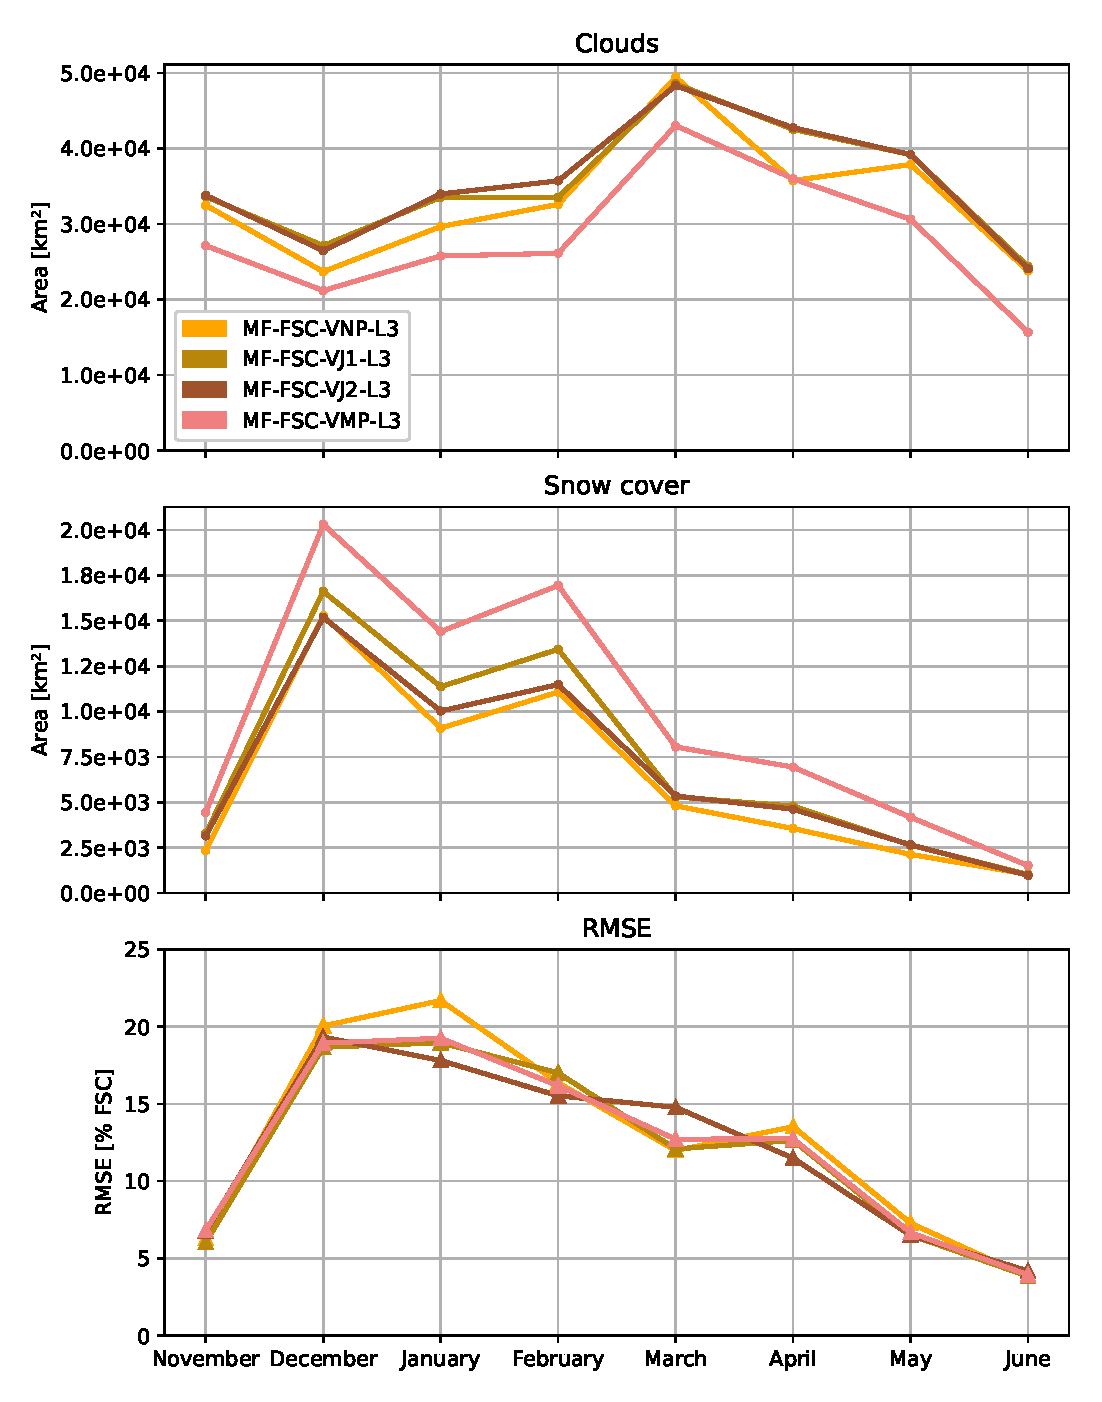
\includegraphics[scale=0.5]{./illustrations/fig05.eps} 
\caption{Per month distribution of:  (a) average daily snow cover area, (b) average daily cloud cover area, and (c)  RMSE with respect to Sentinel-2 reference for winter year 2024/2025, for Météo-France FSC [VIIRS SNPP\textbar JPSS-1\textbar JPSS-2\textbar multi-platform] daily composites. These scores are computed on days when all four products are available.}
\label{fig: multiplatform}
\end{figure}

Figure \ref{fig: multiplatform} summarizes the assessment of the daily compositing of the three VIIRS data sources. Combining SNPP, JPSS-1, and JPSS-2 reduces the overall cloud cover by 16\% compared to using SNPP alone, and by 22\% compared to using either JPSS-1 or JPSS-2 alone. This reduction leads to a substantial increase in mapped snow covered area, with gains of 55\% relative to SNPP alone, 31\% relative to JPSS-1 alone, and 43\% relative to JPSS-2 alone. Furthermore, we find that the multi-platform compositing does not deteriorate the RMSE with respect to each individual product (Fig.~\ref{fig: multiplatform}c).

\DIFaddbegin \subsection{\DIFadd{Comparison with MODIS}}
\label{subsec: res_modis}
\begin{figure}
\centering
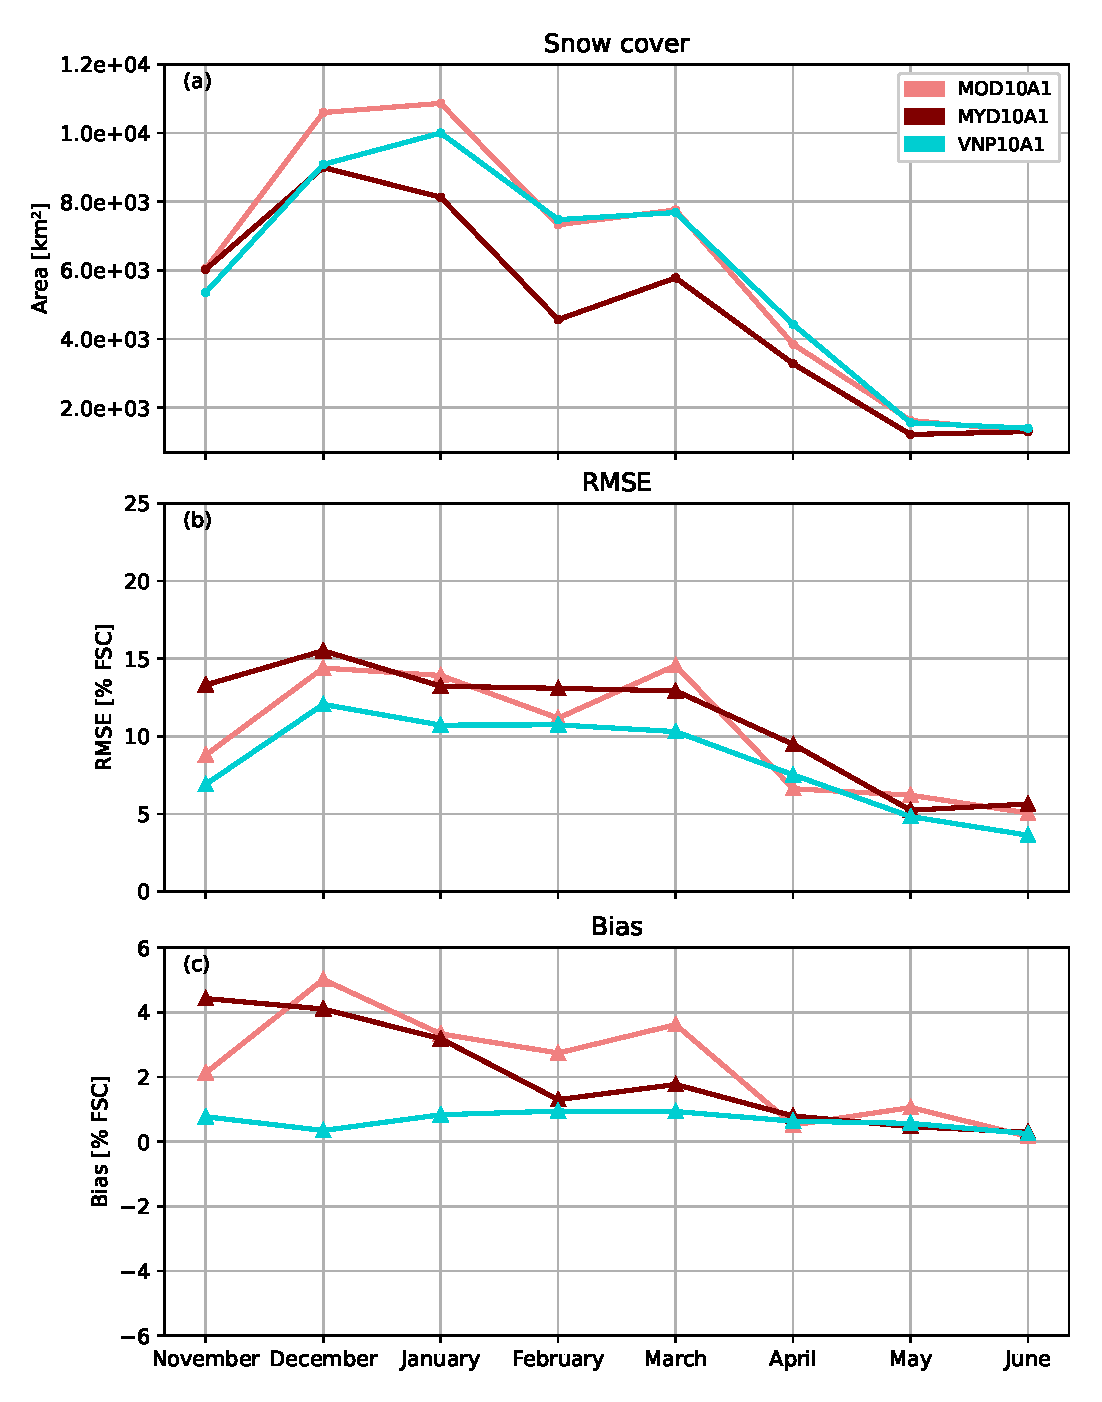
\includegraphics[scale=0.5]{./illustrations/fig06.eps} 
\caption{\DIFaddFL{Per-month distribution of average daily : (a)snow cover area, (b) cloud cover area, (c) RMSE with respect to Sentinel-2, and (d) bias with respect to Sentinel-2  for VNP10A1, MOD10A1 and MYD10A1 on our benchmark for winter year 2023/2024. These scores are computed on days where all four products are available.}}
\label{fig: modis}
\end{figure}

\DIFadd{Figure \ref{fig: modis}a shows a good agreemnt betweeen MOD10A1 and VNP10A1 snow cover area (except for December), whereas MYD10A1 systematically maps less snow. MYD10A1 also detects more clouds than VNP10A1 and MOD10A1 until March, after which VNP10A1 maps more cloud-covered area (Fig. \ref{fig: modis}b). The pixel-to-pixel comparison with Sentinel-2 yields two main results. First, a more positive bias is observed for MODIS than VIIRS, especially during accumulation season. This bias ranges from 2 to 5\% until March for MOD10A1 and until January for MYD10A1, while for VNP10A1 it remains between 0 and 1\% throughout the study period. Second, VNP10A1 exhibits a lower RMSE (Fig. \ref{fig: modis}c) than both MOD10A1 and MYD10A1, with a differences of up to 5\% in March with respect to MOD10A1.
}


\DIFaddend \section{Discussion}
\label{sec: discussion}

\subsection{Sentinel-2 \DIFaddbegin \DIFadd{FSC }\DIFaddend as reference data}
\label{subsec: disc_sentinel2}

\DIFdelbegin \DIFdel{As }\DIFdelend \DIFaddbegin \DIFadd{The use of }\DIFaddend Sentinel-2 FSC \DIFdelbegin \DIFdel{data are freely available at pan-European level, our approach }\DIFdelend \DIFaddbegin \DIFadd{operational product as reference dataset enabled a scalable approach that }\DIFaddend can be easily \DIFdelbegin \DIFdel{scaled and }\DIFdelend replicated in other \DIFdelbegin \DIFdel{mountain regions }\DIFdelend \DIFaddbegin \DIFadd{areas }\DIFaddend of Europe and the mediterranean basin (see Code and Data Availability Statement). \DIFdelbegin \DIFdel{This makes Sentinel-2 snow cover collections a valuable source of reference data to compare to moderate resolution sensors. Many studies used Landsat snow cover products as higher resolution reference \mbox{%DIFAUXCMD
\citep{salomonson_estimating_2004,schwaizer2020SnowCoverExtentb}}\hspace{0pt}%DIFAUXCMD
. However, these products are only available in the United States. In \mbox{%DIFAUXCMD
\citep{schwaizer2020SnowCoverExtentb}}\hspace{0pt}%DIFAUXCMD
, Landsat scenes were manually selected and then processed to produce reference snow cover maps, what can be time consuming. 
}\DIFdelend \DIFaddbegin \DIFadd{These high-resolution products are generated using an NDSI-based algorithm. \mbox{%DIFAUXCMD
\cite{schwaizer2020SnowCoverExtentb} }\hspace{0pt}%DIFAUXCMD
also generated reference snow products from Landsat scenes over the Northern hemisphere via different NDSI-based algorithms. Alternatively, \mbox{%DIFAUXCMD
\cite{rittger_evaluation_2021} }\hspace{0pt}%DIFAUXCMD
employed a spectral unmixing algorithm to retrieve the fractional snow cover area \mbox{%DIFAUXCMD
\citep{painter_retrieval_2009}}\hspace{0pt}%DIFAUXCMD
. This approach is more physically grounded, leverages more spectral bands than the NDSI and open source software are becoming available \mbox{%DIFAUXCMD
\citep{stillinger_landsat_2023, rittger_evaluation_2021, bair_snow_2021}}\hspace{0pt}%DIFAUXCMD
. However, it is also more computationally intensive as it involves solving an optimization problem at the pixel level. For example, \mbox{%DIFAUXCMD
\cite{keuris_adaptive_2023} }\hspace{0pt}%DIFAUXCMD
reported a computation time of 329 s for a single Sentinel-2 scene on a 8 x 1.9 GHz processor with 27 GB RAM. This would be a clear bottleneck in our study where we use 12930 Sentinel-2 products, i.e. potentially up to roughly 9 millions pairs of (pixels,date) to run the endmember inversion algorithm. It also relies on a predefined library of endmembers spectra which may differ across regions and we lack uncertainty estimates of this method applied to Sentinel-2 in Europe (e.g. \mbox{%DIFAUXCMD
\cite{stillinger_landsat_2023, rittger_evaluation_2021, bair_snow_2021}}\hspace{0pt}%DIFAUXCMD
), whereas the uncertainty of the Copernicus FSC products is documented \mbox{%DIFAUXCMD
\citep{barrou_dumont_brief_2021}}\hspace{0pt}%DIFAUXCMD
. Moreover, in a forested region of the western USA, spectral unmixing did not outperform the Copernicus FSC products algorithm in retrieving the fractional snow cover area below the canopy \mbox{%DIFAUXCMD
\citep{muhuri_performance_2021}}\hspace{0pt}%DIFAUXCMD
. 
}

\DIFaddend Snow cover maps from airborne campaigns are another valuable reference data source, but are limited spatially. For example, in \DIFdelbegin \DIFdel{\mbox{%DIFAUXCMD
\citep{stillinger_landsat_2023}}\hspace{0pt}%DIFAUXCMD
, the authors }\DIFdelend \DIFaddbegin \DIFadd{\mbox{%DIFAUXCMD
\cite{stillinger_landsat_2023} }\hspace{0pt}%DIFAUXCMD
}\DIFaddend used the airborne snow observatory dataset, covering an area of 19 000 km² on 6 dates, without considering cloud cover. In this study, we were able to study an area of 105 000 km² with approximately 24 clear-sky observations per pixel. The inevitable shortcoming of our approach is that Sentinel-2 are satellite data and can be affected by the same spatial error patterns \citep{muhuri_performance_2021} that we seek to quantify in this study, despite a much higher resolution than VIIRS products. In particular, snow omission in shaded slopes \citep{gascoin_theia_2019} required recent adaptation on Sentinel-2 pipeline (Sect.~\ref{subsec: data_sentinel2}), and this might contribute to explain the negative difference between VIIRS and Sentinel-2 for Northern aspects we see in Table \DIFdelbegin \DIFdel{\ref{tab: tab04}}\DIFdelend \DIFaddbegin \DIFadd{\ref{tab: tab05}}\DIFaddend . 



\subsection{The enduring legacy of MODIS}
\label{subsec: modis}


\DIFdelbegin \DIFdel{Previous work indicates that NASA VIIRS snow cover products have a similar accuracy to MODIS products \mbox{%DIFAUXCMD
\citep{thapa_cross-comparison_2019, riggs_continuity_2020, zhang_comparative_2020, hall_evaluation_2019}}\hspace{0pt}%DIFAUXCMD
. Our results confirm that the performance of VNP10A1 is similar to the performance previously reported for MOD10A1 in the Alps and the Pyrenees \mbox{%DIFAUXCMD
\citep{ masson_assessment_2018}}\hspace{0pt}%DIFAUXCMD
}\DIFdelend \DIFaddbegin \DIFadd{Figure \ref{fig: modis} suggests that the continuity between  MODIS and VIIRS is globally accomplished, as shown in several works \mbox{%DIFAUXCMD
\citep{riggs_continuity_2020, hall_comparison_2024, rittger_evaluation_2021,zhang_comparative_2020}}\hspace{0pt}%DIFAUXCMD
}\DIFaddend .  

\DIFdelbegin \DIFdel{To verify this more precisely, we compare MOD10A1 and VNP10A1 using the same methodology used throughout this work, except that the images were resampled at 500~m to match the resolution of MOD10A1. We find that both products exhibit a similar performance (Fig. ~\ref{fig: modis}), consistent with previous studies. MOD10A1 product yields more snow than VNP10A1 }\DIFdelend \DIFaddbegin \DIFadd{In terms of snow-covered area, Fig. \ref{fig: modis}a shows more agreement between VIIRS and MODIS aboard Terra, than MODIS aboard Aqua with both other sensors. A major reason for Aqua mapping less snow is a more conservative cloud mask }\DIFaddend (Fig. \DIFdelbegin \DIFdel{~\ref{fig: modis}a), which we attribute to a less restrictive cloud mask. Other studies found an opposite conclusion, i.e. , VIIRS detecting more snowthan MODIS due to a less restrictive cloud mask \mbox{%DIFAUXCMD
\citep{thapa_cross-comparison_2019,liu2022EffectCloudMask, hall_comparison_2024}}\hspace{0pt}%DIFAUXCMD
. However, in  \mbox{%DIFAUXCMD
\citep{thapa_cross-comparison_2019} }\hspace{0pt}%DIFAUXCMD
and \mbox{%DIFAUXCMD
\citep{liu2022EffectCloudMask}}\hspace{0pt}%DIFAUXCMD
, the authors used MYD10A1 products for their comparisons. The RMSE and bias plots in Fig. }\DIFdelend \ref{fig: modis}\DIFdelbegin \DIFdel{b and Figure \ref{fig: modis}cshow that VNP10A1 exhibits a lower RMSE than MOD10A1 in our benchmark. }\DIFdelend \DIFaddbegin \DIFadd{b). This confirms the results of \mbox{%DIFAUXCMD
\cite{liu2022EffectCloudMask} }\hspace{0pt}%DIFAUXCMD
\mbox{%DIFAUXCMD
\cite{thapa_cross-comparison_2019} }\hspace{0pt}%DIFAUXCMD
and can be linked to Aqua MODIS Band 6 defect, which affects snow/cloud discrimination \mbox{%DIFAUXCMD
\citep{riggs2021MODISAquaSnow}}\hspace{0pt}%DIFAUXCMD
. We find a slight positive difference between MOD10A1 and }\DIFaddend VNP10A1 \DIFdelbegin \DIFdel{also shows a smaller bias }\DIFdelend \DIFaddbegin \DIFadd{snow cover fractions (Fig}\DIFaddend . \DIFdelbegin \DIFdel{The slight positive FSC difference between NASA MODIS and VIIRS products has also been observed in \mbox{%DIFAUXCMD
\citep{jacques-hamilton_measurement_2025,stillinger_landsat_2023, liu_consistency_2024}}\hspace{0pt}%DIFAUXCMD
. This deserves a careful examination if }\DIFdelend \DIFaddbegin \DIFadd{\ref{fig: modis}c), which is consistent with previous studies \mbox{%DIFAUXCMD
\cite{jacques-hamilton_measurement_2025,stillinger_landsat_2023,liu2022EffectCloudMask,keuris_adaptive_2023}}\hspace{0pt}%DIFAUXCMD
. We find a similar positive bias for MYD10A1 from December to January. Aqua overpass time (approximately 2pm at the end of 2023) is closer to SNPP overpass (1:30 pm) time than Terra’s (approximately 10am at the end of 2023), therefore this difference cannot be solely due to intra-day snow cover variations. This results highlight the need to cross calibrate }\DIFaddend MODIS and VIIRS products \DIFdelbegin \DIFdel{are to be merged to generate a long term record. For snow related applications, VIIRS data improve MODIS in }\DIFdelend \DIFaddbegin \DIFadd{should they be merged into a long-term record. NASA’s VIIRS products slightly outperforms their MODIS counterparts in terms of RMSE (Fig. 6d), what can be explained by its higher }\DIFaddend spatial resolution (375~m vs 463~m)\DIFdelbegin \DIFdel{and }\DIFdelend \DIFaddbegin \DIFadd{. Aggregated to 500 m, the uncertainty of VNP10A1 is reduced, while the same is not valid for MODIS. Also, VIIRS data improve MODIS in }\DIFaddend reliability at high viewing angles\DIFaddbegin \DIFadd{, }\DIFaddend as MODIS effective pixel size increases dramatically towards the edges of the swath \citep{dozier2008TimeSpaceContinuity}. This effect \DIFdelbegin \DIFdel{can be }\DIFdelend \DIFaddbegin \DIFadd{has been }\DIFaddend taken into account when using MODIS data in snow modeling \DIFaddbegin \DIFadd{by some authors }\DIFaddend \citep{sun_evaluation_2024}. On the other hand, VIIRS instrument is designed to limit pixel size growth towards the border of the swath. For comparison, the effective spatial resolution at the edge of scan is 0.74x0.74~km² for VIIRS I-bands (375~m at nadir) while it is 1x3~km² for MODIS 500~m bands \citep{schueler_viirs_2013}. Here, we find that VIIRS snow \DIFdelbegin \DIFdel{products accuracy is strongly }\DIFdelend \DIFaddbegin \DIFadd{detection is }\DIFaddend affected by the view zenith angle only above 60° \DIFaddbegin \DIFadd{(panels 5a to 5c of Figure \ref{fig: synthesis})}\DIFaddend . This effect \DIFdelbegin \DIFdel{affects }\DIFdelend \DIFaddbegin \DIFadd{concerns }\DIFaddend approximately one out of nine pixels, as inferred from panel 5d of Figure \ref{fig: synthesis}, where about half a million pixels fall into the $>$ 60° category out of a total of 4.89 million match-ups for MF-FSC-VNP-L3 (Table~\DIFdelbegin \DIFdel{\ref{tab: tab03}}\DIFdelend \DIFaddbegin \DIFadd{\ref{tab: tab05}}\DIFaddend ). This result is encouraging for downstream applications such as data assimilation, as it suggests that most observations can be treated consistently regardless of the sensor zenith angle. However, in \citep{stillinger_landsat_2023} the authors reported substantial errors at zenith angles as low as 40°, indicating that this finding should be confirmed by further studies.


\DIFdelbegin %DIFDELCMD < \begin{figure}
%DIFDELCMD < \centering
%DIFDELCMD < 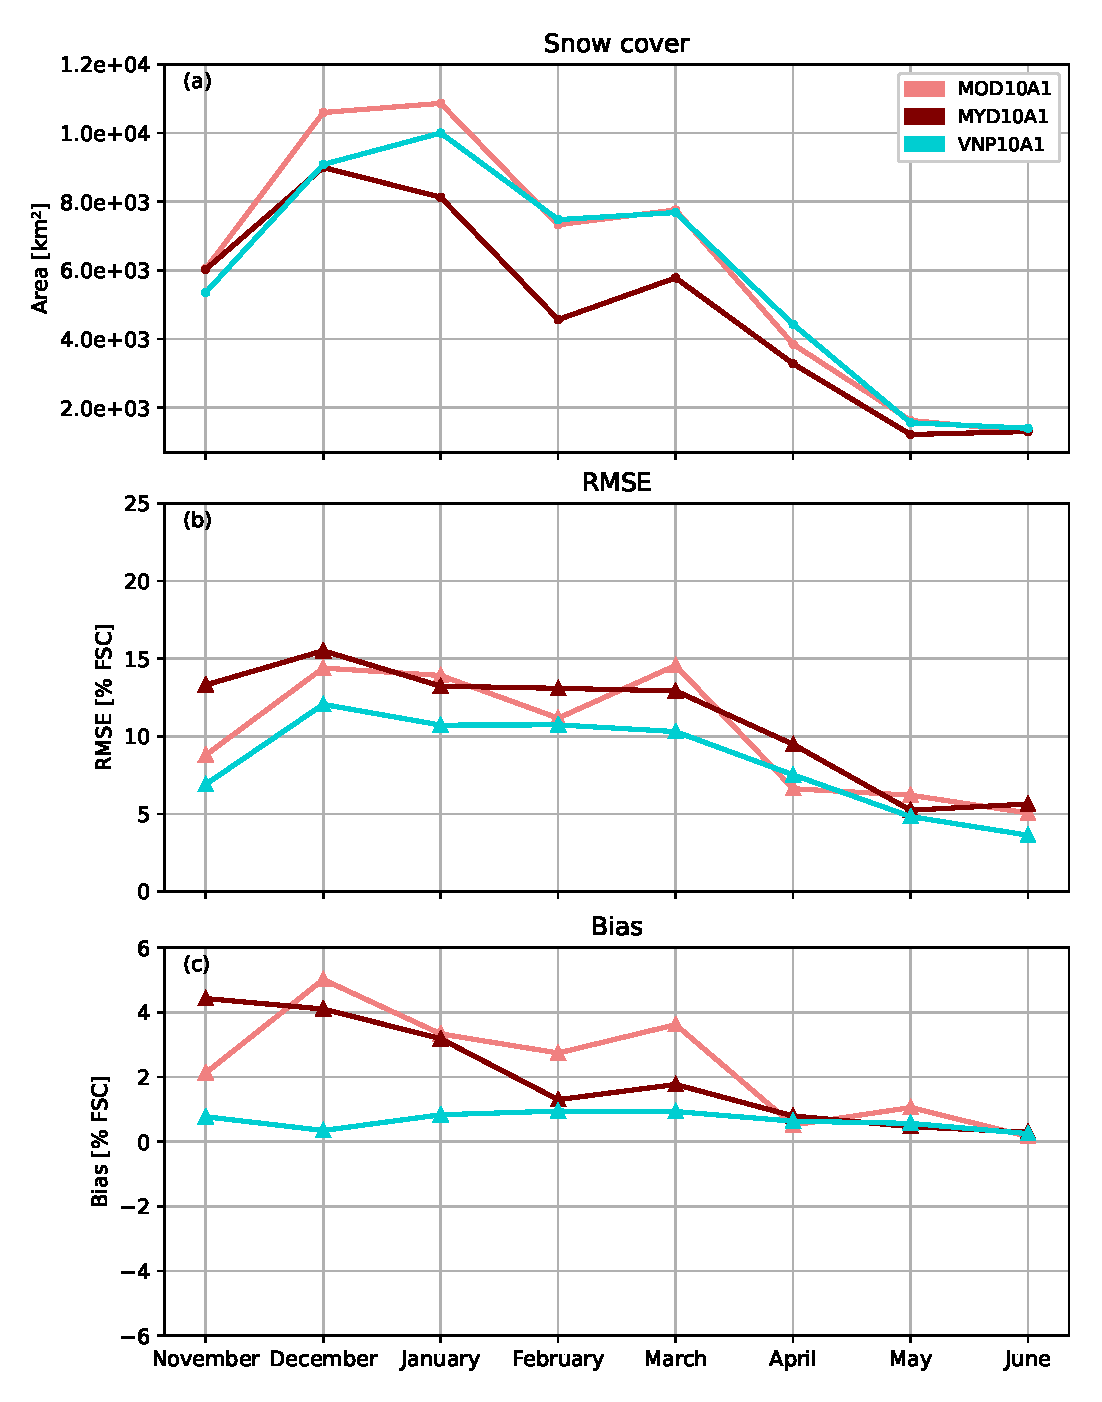
\includegraphics[scale=0.5]{./illustrations/fig06.eps} 
%DIFDELCMD < %%%
%DIFDELCMD < \caption{%
{%DIFAUXCMD
\DIFdelFL{Per-month distribution of: (a) average daily snow cover area, (b) RMSE with respect to Sentinel-2 reference, and (c) bias with respect to Sentinel-2 reference for VNP10A1 and MOD10A1 products on our benchmark for winter year 2023/2024. These scores are computed on days where all four products are available.}}
%DIFAUXCMD
%DIFDELCMD < 

%DIFDELCMD < \label{fig: modis}
%DIFDELCMD < \end{figure}
%DIFDELCMD < 

%DIFDELCMD < %%%
\DIFdelend \subsection{FSC error heteroscedasticity} 

Heteroscedasticity denotes situations in which the error variance of a variable is not constant and varies as a function of one or more explanatory variables. In geosciences, the term is often used to describe spatial variability in error variance that can be linked to surface properties \citep{hugonnet2022UncertaintyAnalysisDigital}. In \citep{aalstad_evaluating_2020}, we can find a study of heteroscedasticity in the context of fractional snow cover. The authors showed that FSC errors depend on FSC itself and proposed a correction of error variance based on a corrective factor and FSC value. A similar non stationary behavior has been reported in many evaluations of satellite-derived snow cover products \citep{jacques-hamilton_measurement_2025, stillinger_landsat_2023, schwaizer2020SnowCoverExtentb}.
FSC is a double-bounded variable, and its variance is constrained near the limits of its range. For instance, in Fig. \ref{fig: synthesis}, panel 1c, the error distribution becomes increasingly asymmetric as FSC approaches its bounds (reference classes 1–25\% and 76–99\%). This means that FSC variance depends less on the FSC value itself and more on the proximity to the boundaries: when a bound lies closer than the natural spread of the variable, the variance is effectively reduced. Beyond this intrinsic behavior, FSC variance is also influenced by multiple external factors and a key aim of evaluation studies is to characterize these variations—that is, to quantify heteroscedasticity in a broad sense. Recent work \citep{hugonnet2022UncertaintyAnalysisDigital} highlights that properly handling heteroscedasticity is essential for propagating remote sensing uncertainties into downstream applications. Explicitly modeling heteroscedastic errors could therefore be highly beneficial in data assimilation studies, which typically assume a fixed observation error variance \citep{baba_assimilation_2018}.


\subsection{Mixed pixels}
\DIFaddbegin \label{subsec: mixed_pixels}
\DIFaddend 

To further investigate the behavior of VIIRS FSC products in mixed pixels, we compare the NDSI from VNP10A1 and the FSC from Sentinel-2 in forested and non-forested areas. We plot all the correspondences in a scatter plot (Fig. \ref{fig: scatter}), compute correlation scores and fit a linear model to predict FSC given an NDSI. The details about this scatter analysis are reported in Appendix \ref{subsec: ndsi_fit}. The linear fit of Figure \ref{fig: scatter} in open areas is remarkably close to the one proposed in \citep{salomonson_development_2006}, although this relationship was calculated for MODIS data using Landsat as reference, while in forested areas the linear model exhibits a steeper slope (\DIFdelbegin \DIFdel{2.14 compared to 1.39 }\DIFdelend \DIFaddbegin \DIFadd{2.17 compared to 1.43 }\DIFaddend in open areas). For FSC values higher than 20\%, our fit is close to a sigmoid function previously optimized for Sentinel-2, assuming a 50\% tree cover density \citep{gascoin_estimating_2020}. 
The Pearson correlation coefficient $r$ suggests good (open, $r=0.75$) to moderate (forest $r=0.56$) correlation between NDSI and FSC values in mixed pixels. This results in a larger mean error when fitting a linear model, as reflected by the low $R^2$ value (\DIFdelbegin \DIFdel{0.32 }\DIFdelend \DIFaddbegin \DIFadd{0.31 }\DIFaddend in forests). In other words, enforcing a linear relationship between two weakly correlated variables inevitably introduces substantial uncertainty when estimating FSC in mixed pixels. This analysis explains the results reported in panel 1a-c of Figure \ref{fig: synthesis} and in Table \DIFdelbegin \DIFdel{\ref{tab: tab04} }\DIFdelend \DIFaddbegin \DIFadd{\ref{tab: tab05} }\DIFaddend showing RMSE for mixed pixels typically between 20 and 30\%, while it is generally 10-15\% when calculated over all correspondences. Estimating the snow covered fraction within a pixel is inherently challenging because it is an attempt to infer information at a scale finer than the sensor’s spatial resolution. Yet, this information is relevant for many applications (e.g., snowline estimation and late season snow patches distribution mapping) and errors in space-borne fractional estimates can still be significantly smaller than uncertainties in snow cover models \citep{girotto_data_2020} and useful to refine snow cover analyses  \citep{aalstad_evaluating_2020}. Numerous methods have been proposed to address this problem, in particular spectral unmixing techniques \citep{painter_retrieval_2009}. Nonetheless, only NDSI-based techniques are, to date, operational at the global scale, and, therefore, it is important to understand how the selected NDSI-FSC regression affects the accuracy of a product. A user wishing to exploit the FSC information in V[NP\textbar J1]10A1 must apply a conversion model for the NDSI values given in the NDSI\_Snow\_Cover variable (Sect.~\ref{subsec: data_nasa}). The FRA6T linear relationship \citep{salomonson_development_2006} is often chosen for this transformation \citep{stillinger_landsat_2023,masson_assessment_2018}. We confirm that this choice is appropriate for VNP10A1 outside forested areas in our domain. \DIFaddbegin \DIFadd{We also tested the fit obtained in Fig. \ref{fig: scatter}. We repeated all steps outlined in Section \ref{subsec: meth_resampling} but with the NDSI-to-FSC coversion found in Fig. \ref{fig: scatter}, differentiating forest and open ralationships. However, we found no added value in this approach: the overall performance was equivalent in open areas and degraded in forests (not shown). This confirms that developing predictive models for NDSI-to-FSC conversion across varying seasons and terrain is challenging and requires substantial work beyond our current scope.
}\DIFaddend 

\begin{figure}
\centering
\DIFdelbeginFL %DIFDELCMD < 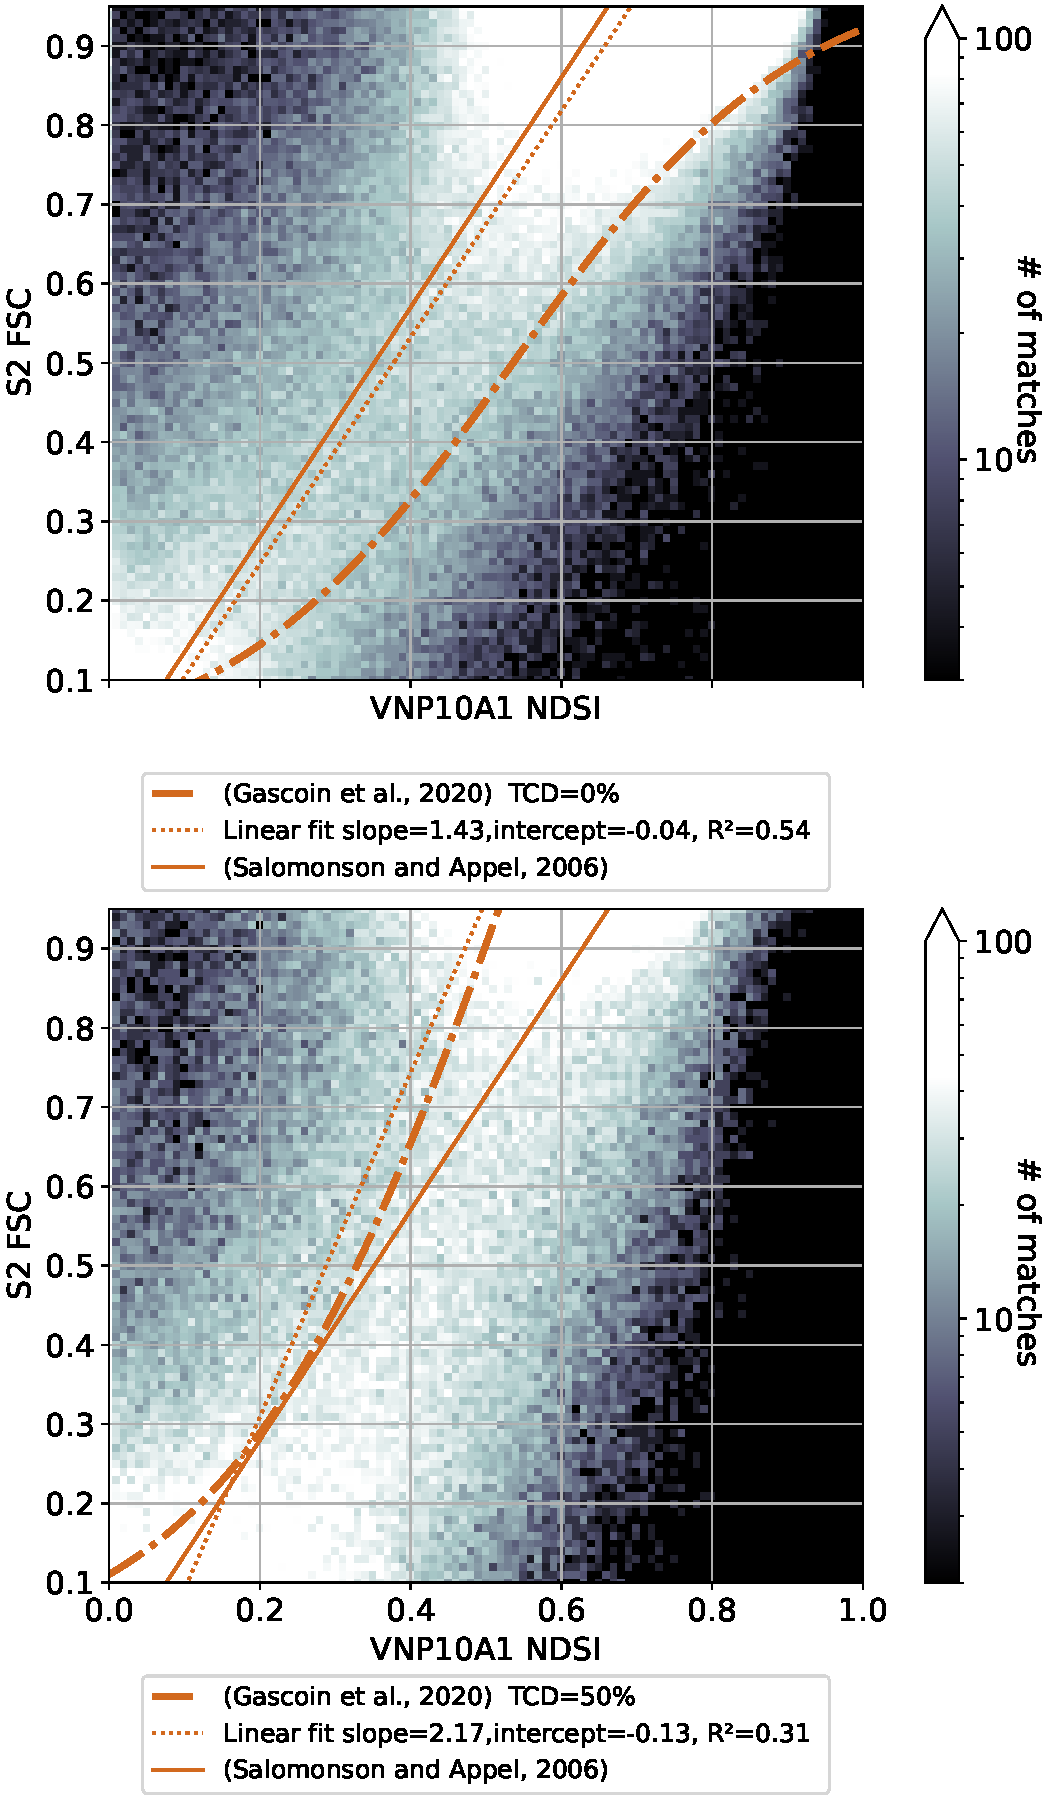
\includegraphics[scale=0.35]{illustrations/fig07.pdf}
%DIFDELCMD < %%%
\DIFdelendFL \DIFaddbeginFL 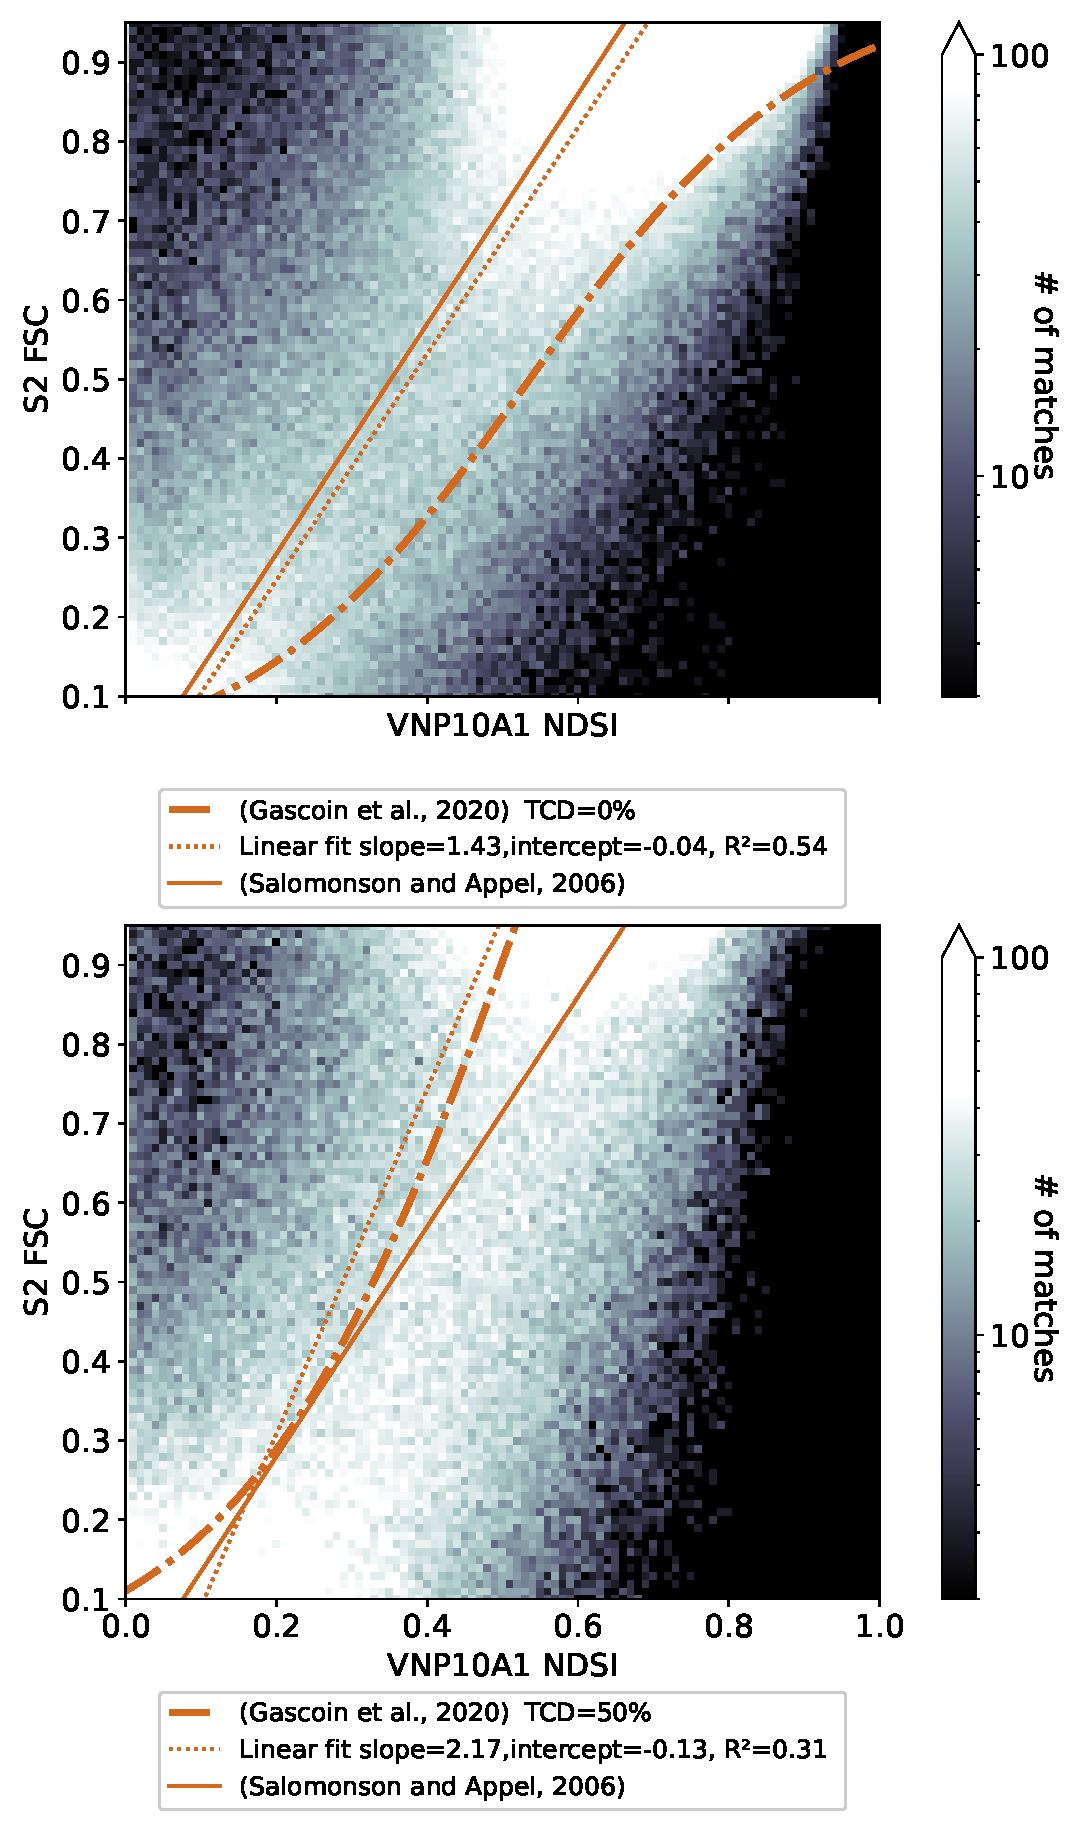
\includegraphics[scale=0.35]{illustrations/fig07.eps}
\DIFaddendFL \caption{Scatter plot of VNP10A1 NDSI versus Sentinel-2 reference FSC. The colormap represents the number of match-ups per $(\mathrm{NDSI_{OBS}}, \mathrm{FSC_{REF}}$) pair. The dashed line is the linear fit. The dash-dotted line is the sigmoid tree cover density corrected fit used in \citep{gascoin_estimating_2020}. The solid line is the relationship of \citep{salomonson_development_2006} for MODIS using Landsat as reference. We used a logarithmic colormap between the 20th and 90th percentiles of the data distribution. The methodological details are given in Appendix \ref{subsec: ndsi_fit}}
\label{fig: scatter}
\end{figure}

\subsection{Forest\DIFdelbegin \DIFdel{and }\DIFdelend \DIFaddbegin \DIFadd{, }\DIFaddend topography \DIFaddbegin \DIFadd{and clouds}\DIFaddend }

In our benchmark, VIIRS snow cover estimations in forested areas present higher uncertainty and a negative bias (omissions) compared with Sentinel-2 (Fig.~\ref{fig: synthesis}, Table~\DIFdelbegin \DIFdel{\ref{tab: tab04}}\DIFdelend \DIFaddbegin \DIFadd{\ref{tab: tab05}}\DIFaddend ). While reduced precision under canopy cover is a common outcome \citep{stillinger_landsat_2023, muhuri_performance_2021, rittger2020CanopyAdjustmentImproved}, the observed negative bias might stem from the forest adjustment applied to the Sentinel-2 reference $\mathrm{FSC_{OG}}$ (see Sect.~\ref{subsec: data_sentinel2}). This correction increases the reference FSC relative to what is measured if only NDSI was taken into account. In contrast, no canopy adjustment is applied to the VIIRS products considered in this study \citep{rittger2020CanopyAdjustmentImproved}. Conversely, the influence of topography on spaceborne snow cover retrievals has been less investigated \citep{rittger_evaluation_2021}. In this study, we show that aspect plays a key role in snow cover detection in the mountains. Indeed, in the Northern Hemisphere, the local sun angle is lower for Northern slopes than Southern ones. In winter, little or no sunlight reaches these slopes. Thus, the snow detection relies heavily on diffused light. In \citep{keuris_adaptive_2023}, the authors illustrated how NDSI values for snow-free areas can be higher in the shadow, potentially causing false detection. \DIFdelbegin \DIFdel{In our benchmark, we found }\DIFdelend \DIFaddbegin \DIFadd{Low visible reflectance screens are generally implemented in snow cover retrieval algorithms to limit this issue. Both target and reference dataset pipelines implement a low reflectance screen with fixed thresholds. We find }\DIFaddend the error to be dominated by omissions in Northern slopes (Table~\DIFdelbegin \DIFdel{\ref{tab: tab04}). This can be due to the reflectance of the red (I1) VIIRS band that we implemented in the MF-FSC-VMP-L3 pipeline (see Appendix \ref{app: mf_product}) to limit false detection , that might also introduce omissions when solar illumination is weak or absent. However, it should be noted that our reference is satellite-based as well and suffers from similar problems. Indeed}\DIFdelend \DIFaddbegin \DIFadd{\ref{tab: tab05}), what suggests that the combined effect of both target and reference screens and relative thresholds results in VIIRS being more conservative in snow detection of shaded slopes. In particular}\DIFaddend , the shadowed slope correction applied to Sentinel-2 products (Sect.~\ref{subsec: data_sentinel2}) might \DIFdelbegin \DIFdel{as well }\DIFdelend contribute to explaining the observed difference. \DIFaddbegin \DIFadd{Locally-adaptive thresholds have been proposed to address this issue.  \mbox{%DIFAUXCMD
\cite{schwaizer2020SnowCoverExtent} }\hspace{0pt}%DIFAUXCMD
adopted spatially (latitude and elevation) and temporally (monthly) varying NDSI thresholds for a VIIRS based Northern Hemisphere product (see Table \ref{tab: tab02}). \mbox{%DIFAUXCMD
\cite{zhang_comparative_2020} }\hspace{0pt}%DIFAUXCMD
optimized VNP10A1 NDSI thresholds for each in situ snow depth station in a China-based study. However, they also found non-significant correlations with several geographic and meteorological variables, suggesting that is hard to predict the distribution of an optimal NDSI threshold. A further challenge in snow cover retrieval is snow-cloud discrimination. In this study, we mitigated the influence of cloud masking by using the union of cloud masks from both reference and target datasets. Our results show greater consistency in cloud masking for VIIRS products (Fig. \ref{fig: multiplatform}), where the same Météo-France algorithm is applied, compared to MODIS products (Fig. \ref{fig: modis}), where Terra and Aqua use slightly different algorithms due to the afore-mentioned Aqua Band 6 issue \mbox{%DIFAUXCMD
\citep{riggs2021MODISAquaSnow}}\hspace{0pt}%DIFAUXCMD
. However, we did not perform a detailed comparison of cloud masking across different product sources, as addressed in other studies \mbox{%DIFAUXCMD
\citep{liu2022EffectCloudMask}}\hspace{0pt}%DIFAUXCMD
.
}\DIFaddend 





\subsection{VIIRS data fusion}
\label{subsec: disc_multiplatform}

The results in Section \ref{subsec: res_composite} indicate that JPSS-2 snow cover retrievals are consistent with those from SNPP and JPSS-1. Although this assessment is based on the Météo-France multi-platform composite product, that is not distributed globally, the results support broader conclusions about the continuity and reliability of VIIRS snow cover measurements across platforms. It is reasonable to expect that the NASA snow cover product for JPSS-2 observations, once distributed \citep{riggs2023viirs}, will show similar performance to VNP10A1 and VJ110A1. The availability of three interchangeable sensors naturally lends itself to fusion techniques that exploit the complementarity among the VIIRS platforms.  
Results in Section \ref{subsec: res_composite} confirm the benefits of this approach: combining the three observations, acquired about 50 minutes apart, increases the amount of exploitable data\DIFdelbegin \DIFdel{as }\DIFdelend \DIFaddbegin \DIFadd{. }\DIFaddend clouds move over the course of the day. These estimations are aligned with recent work that proposes daily composites of MODIS and VIIRS observations  \citep{dietz_brief_2025}. \DIFaddbegin \DIFadd{This improvement in data availability from multi-platform compositing likely arises from a combination of mechanisms. Cloud advection over the \~50-minute window between overpasses can displace cloud features by ~30 km (based on typical wind speeds of ~10 m/s), reducing cloud cover in composites. Differences in viewing geometry may also contribute, as cloud shadow effects scale with cloud height (typically 5–10 km). While our preliminary estimates suggest cloud advection is the dominant mechanism. While our preliminary estimates suggest cloud advection is the dominant mechanism, viewing geometry effects (and other phenomena we have not included here) may also play significant roles under certain conditions. A full attribution would require dedicated analysis beyond the scope of this study. }\DIFaddend Several fusion strategies can be used to combine observations from the three VIIRS platforms. In this study, we adopt a simple yet effective criterion based on the view zenith angle (Sect.~\ref{subsec: meth_compo}). More advanced approaches could be envisaged to further increase the number of clear observations and/or improve product accuracy. For instance, in  the authors propose retaining only pixels consistently classified across platforms, while the NSIDC VIIRS composites (V[NP\textbar J1]10A1) rely on the phase angle (i.e. the difference between view and solar zenith angles) to account jointly for view and illumination conditions, both of which significantly influence snow reflectance and hence the NDSI \citep{ji2022NewIndexSnow}. 

\conclusions  %% \conclusions[modified heading if necessary]
\label{sec: conclusion}

We evaluated the performance of VIIRS snow products over a large region encompassing several mountain ranges in France using Sentinel-2 snow products as reference. This allowed us to compute robust error statistics in various configurations of land cover, topography and sensor geometry. For V[NP \textbar J1]10A1, we estimate the RMSE to be about 10\% and the bias to be close to zero. The MF-FSC-VMP-L3 product exhibits a higher RMSE of about 15\%, meaning that there is still room for algorithm improvement, especially in forested areas. Regarding binary metrics about snow occurrence the three products show similar \DIFdelbegin \DIFdel{accuracy (96-98\%) and }\DIFdelend $\mathrm{F_1}$ score (\DIFdelbegin \DIFdel{92-93}\DIFdelend \DIFaddbegin \DIFadd{89-92}\DIFaddend \%). We show that global statistics hide a complex error dynamic with the RMSE that can rise as high as 30\% and \DIFdelbegin \DIFdel{accuracy }\DIFdelend \DIFaddbegin \DIFadd{$\mathrm{F_1}$ }\DIFaddend that can drop to \DIFdelbegin \DIFdel{0.76}\DIFdelend \DIFaddbegin \DIFadd{75\%}\DIFaddend . This dynamic is mainly driven by land cover (mixed pixels, forest) and topography (slope angle and orientation). This study suggests that a stratified error model should be considered in downstream applications such as data assimilation to properly account for uncertainties. Our assessment suggests that the platforms composing the VIIRS constellation (SNPP, JPSS-1 and JPSS-2) have an overall comparable performance. In particular, SNPP and JPSS-1 perform consistently with each other across a wide variety of slopes, and viewing conditions, while preliminary results for JPSS-2 products suggest that the interchangeability with the other VIIRS platforms is largely achieved. The availability of three comparable phase-shifted VIIRS platforms naturally opens towards data fusion techniques to address cloud cover by taking advantage of the complementarity of multiple satellite passes. We show how these fusion techniques can reduce cloud cover of operational snow products by 15-20\%. \DIFdelbegin \DIFdel{Our results confirm for the France mountains the }\DIFdelend \DIFaddbegin \DIFadd{Furthermore, we found that VIIRS data quality are is at least as good as MODIS, with MODIS exhibiting a higher RMSE of up to 5\%. The }\DIFaddend quality and robustness of VIIRS \DIFdelbegin \DIFdel{snow cover observations already emphasized by the studies reviewed in this article. The next step is to prepare the }\DIFdelend \DIFaddbegin \DIFadd{observations -already emphasized by other sutdies- are well-estabilished and VIIRS snow cover products can take over from MODIS. We recommend preparing }\DIFaddend concerned applications for the transition \DIFdelbegin \DIFdel{from MODIS before it }\DIFdelend \DIFaddbegin \DIFadd{the before MODIS }\DIFaddend is decommissioned. In this context, our future work will focus on the assimilation of Météo-France FSC VIIRS multi-platform daily composite into a snowpack model. 



\codedataavailability{The regridded V[NP\textbar J1]10, MF-FSC-V[MP\textbar NP\textbar J1\textbar J2]-L3 datasets over French mountain ranges used in this study are available in  \cite{imperatore_2026_18157029}.
The code developed for the processing and analysis, and the generation of figures and tables in this article is available in \cite{imperatore_2026_18773106}. } %% use this section when having data sets and software code available


%\sampleavailability{TEXT} %% use this section when having geoscientific samples available


%\videosupplement{TEXT} %% use this section when having video supplements available

\clearpage 

\appendix
\section{Météo-France VIIRS fractional snow cover algorithm}
\label{app: mf_product}
%% Appendix A

We describe hereby the data processing pipeline for Météo-France FSC VIIRS multi-platform daily composite. This operational product is a composition of the snow cover observations of the VIIRS mission over metropolitan France. The data processing pipeline is illustrated in Fig. \ref{fig: cms_product}.

The NOAA VIIRS Sensor Data Record (SDR) products are collected via local acquisition in real-time (10-15' after satellite pass). These products are reprojected from swath geometry to the output grid in geographic coordinates using Satpy's resampling \citep{martin_raspaud_2025_17552484} swath data resampling method with nearest neighbour interpolation. The snow detection algorithm, applied to every new acquisition, consists of the following steps. First, the NDSI is computed for each pixel using Imagery bands 01 and 03. Pixels with NDSI $>$ 0 and red band reflectance $>$ 0.07 are classified as snow covered. Next, we apply a screen based on the pseudo RGB composite for snow detection presented in \citep{vidot_daytime_2017}. This is an internal product where R,G,B bands are a linear combination of VIIRS M-bands optimized for weather forecasters to qualitatively estimate snow cover extent and duration. In this product, the snow signal is stronger in the red band. This is used to create a false detection filter that follows the following steps. First, we identify pixels where there is a very strong snow signal by setting a threshold of 40\% of distance from the red in the RGB color space. Since our image is encoded in bytes, this is equivalent to keeping all points that have a distance smaller than 102 from the triplet (255,0,0) in the RGB color space. Then we find a "possible snow" around these pixels by performing an Euclidean Distance Transform with a radius of 17 pixels (=~6.375~km). This "possible snow" mask is then applied to the positive NDSI image to exclude pixels previously detected as snow. These steps can be seen as a quick way to eliminate physically unlikely false detection that arises when using only the thresholds on the NDSI and the red band. Open and inland water masks are computed from CORINE Landcover 2006 dataset and applied in order to give contextual information. Finally, the cloud mask is computed using the MAIA pipeline \citep{lavanat_maia_2018} and applied to generate the final snow cover map. At the end of each day, the snow cover maps generated from the three satellite acquisitions are fused to produce a daily composite using the observations of all platforms. For each VIIRS acquisition, we also create a sensor zenith angle map. It is obtained from the geolocation files, the VIIRS Image Bands SDR Ellipsoid Terrain Corrected Geolocation product (GITCO - SDR), and projected using the same swath reprojection algorithm applied to the snow cover data. The composition algorithm takes as input the snow cover sensor zenith angle maps of one day over the product domain. The algorithm first selects for each pixel the pass with lower zenith angle. Then, it partially fills cloud and data gaps by iteratively taking higher zenith angle observations if valid. It should be noted that no assumption is made on the different platforms' data quality and the only criteria is the sensor zenith angle, hypothesis that is supported by the evaluation shown in Section \ref{subsec: disc_multiplatform}. This product is composed of three layers: snow\_cover\_fraction, the result of the algorithm explained herein, sensor\_zenith\_angle and platform the report information on the origin of the observation corresponding to a pixel, allowing the user to track discontinuities.
The validation of this approach for daily composition is illustrated in Section \ref{subsec: disc_multiplatform}.

\appendixfigures
\begin{figure}
\centering
\includegraphics[scale=0.14]{./illustrations/fig08.pdf} 
\caption{Block diagram of the Météo-France FSC VIIRS multi-platform daily composite pipeline.}
\label{fig: cms_product}
\end{figure}

\section{Correlation of VIIRS NDSI with Sentinel-2 FSC}
\label{subsec: ndsi_fit}

To evaluate the ability of VIIRS products to represent a snow cover fraction on mixed pixels, we perform a scatter analysis between VIIRS NDSI measures and Sentinel-2 reference FSC. We compute the Pearson correlation coefficient as in Eq. \eqref{eq: pearson},
\begin{equation}
    r = \frac{
    N~\sum_{i=0}^{N} ~ x_i ~ y^*_i 
    - \sum_{i=0}^{N} x_i \sum_{i=0}^{N} y^*_i }{
    \sqrt{N \sum_{i=0}^{N} x_i^2 - (\sum_{i=0}^{N} x_i)^2}
    \sqrt{N \sum_{i=0}^{N} {y^*_i}^2 - (\sum_{i=0}^{N} y^*_i)^2}}
\label{eq: pearson}
\end{equation}
where we used $x_i$ to refer to the VIIRS NDSI values and $y^*_i$ for the reference Sentinel-2 FSC. This allows us understand the use of Eq. \ref{eq: salomonson_appel} is justified for FSC extraction from NDSI for VIIRS data on our study area. Additionally, we perform a linear fit using all the correspondences available on our study area between VIIRS NDSI and Sentinel-2 reference FSC.  Following the approach depicted in \citep{salomonson_estimating_2004}, we fit the model $\mathrm{NDSI}=a'~\mathrm{FSC} + b'$ minimizing NDSI deviations rather than minimizing FSC deviations on a FSC model ($\mathrm{FSC}=a~\mathrm{NDSI} + b$).
\begin{equation}
min_{a',b'} \sum_{i=0}^{\bar{N}} [(a'~y^*_i+b') - x_i]^2
\label{eq: regression}
\end{equation}
We find the coefficients $a,b$ by inversion: $a=\frac{1}{a'}$ and $b=-b'$. Fitting on NDSI deviations ensures a higher $a$ coefficient and therefore a higher sensitivity of FSC to NDSI, that is a desirable feature of the model \citep{salomonson_estimating_2004}. Since this is a linear least square regression with a single independent variable, the coefficient of determination ($R^2$ score) of our fit is defined as square of the Pearson correlation coefficient (Eq. \ref{eq: pearson}). The fit was obtained using least square minimization and considering all the $\bar{N}$ correspondences with a FSC between 10\% and 95\% as suggested in \citep{salomonson_development_2006}.


\noappendix       %% use this to mark the end of the appendix section. Otherwise the figures might be numbered incorrectly (e.g. 10 instead of 1).

%% Regarding figures and tables in appendices, the following two options are possible depending on your general handling of figures and tables in the manuscript environment:

%% Option 1: If you sorted all figures and tables into the sections of the text, please also sort the appendix figures and appendix tables into the respective appendix sections.
%% They will be correctly named automatically.

%% Option 2: If you put all figures after the reference list, please insert appendix tables and figures after the normal tables and figures.
%% To rename them correctly to A1, A2, etc., please add the following commands in front of them:

%\appendixfigures  %% needs to be added in front of appendix figures

%\appendixtables   %% needs to be added in front of appendix tables

%% Please add \clearpage between each table and/or figure. Further guidelines on figures and tables can be found below.



\authorcontribution{SGa, ML and NI designed the study. NI developed performed the study under the supervision of SG, ML and MD. MD and NI designed the MF-FSC algorithm and SGu implemented the operational pipeline. AM processed the MF-FSC-L3 data for this research. JBH coordinated the technical resources for the MF-FSC-L3 product. NI and SG wrote the paper with the help of ML, SGu and MD. All authors contributed to results analysis and discussion.} %% this section is mandatory


\competinginterests{Regarding conflicts of interest, we only need to mention that Marie Dumont belongs to the editorial team of The Cryosphere.} %% this section is mandatory even if you declare that no competing interests are present

%\disclaimer{TEXT} %% optional section

\begin{acknowledgements}
This research is part of a PhD funded by Centre National d’Études Spatiales (CNES) and Météo-France. It also receives financial support from CNES, France (ROR: https://ror.org/04h1h0y33 ) through the TRISHNA-Cryosphere project. This paper receives contributions from Marie Dumont funded by the European Research Council (ERC) under the European Union’s Horizon 2020 research and innovation program (IVORI; grant no. 949516).
CNRM/CEN is part of LabEX OSUG@2020. It was carried out using Météo-France’s and CESBIO computational and human resources. We gratefully acknowledge Mathieu Fructus for his expertise and Zacharie Barrou Dumont for the fruitful discussions on satellite fractional snow cover error characterization
\end{acknowledgements}




%% REFERENCES

\bibliographystyle{copernicus}
\bibliography{references}





\end{document}
